%%%%%%%%%%%%%%%%%%%%%%%%%%%%%%%%%%%%%%%%%%%%%%%%%%%%%%%%%%%%%%%%%%%%%%
% Lớp 12 | Tọa độ của véc-tơ trong không gian | Véc-tơ và các phép toán véc-tơ trong không gian (chưa tọa độ hóa)
% Dạng 2H2?1-3: Tích vô hướng và ứng dụng
% Số câu: 40  (sinh tự động bởi tach_cau.py; từ nay thầy sửa trực tiếp file này)
%%%%%%%%%%%%%%%%%%%%%%%%%%%%%%%%%%%%%%%%%%%%%%%%%%%%%%%%%%%%%%%%%%%%%%

%%%%%%%%%%%%%%%% TRẮC NGHIỆM 4 PHƯƠNG ÁN %%%%%%%%%%%%%%%%

% nguồn: Lop_12_Hinh_hoc_Chuong_2
\begin{ex}%[2H2N1-3]%[ma:7b3dc5eb]
	Cho hai vectơ $\overrightarrow{a}$ và $\overrightarrow{b}$ khác $\overrightarrow{0}$.  Xác định góc $\alpha$ giữa hai vectơ $\overrightarrow{a}$ và $\overrightarrow{b}$ khi $\overrightarrow{a}\overrightarrow{b} = -\left|\overrightarrow{a}\right|\cdot\left|\overrightarrow{b}\right|$.
	\choice 
		{\True $\alpha  = 180^\circ$}
		{$\alpha =  0^\circ$}
		{$\alpha = 90^\circ$} 
		 {$\alpha = 45^\circ$}
	 \loigiai{
		Ta có $\overrightarrow{a}\cdot\overrightarrow{b}  = \left|\overrightarrow{a}\right|\cdot\left|\overrightarrow{b}\right|\cos\left(\overrightarrow{a},\overrightarrow{b}\right)$.\\
		Mà theo giả thiết $\overrightarrow{a}\cdot\overrightarrow{b} = -\left|\overrightarrow{a}\right|\cdot\left|\overrightarrow{b}\right|$ nên $\cos\left(\overrightarrow{a},\overrightarrow{b}\right) =  -1 \Rightarrow \left(\overrightarrow{a},\overrightarrow{b}\right) = 180^\circ$.
	 }
\end{ex}

% nguồn: Lop_12_Hinh_hoc_Chuong_2
\begin{ex}%[2H2N1-3]%[ma:b6031aab]
	Cho hình lập phương $ABCD.EFGH$. Hãy xác định góc giữa cặp vectơ $\overrightarrow{AB}$ và $\overrightarrow{EG}$? 
	\choice 
		{$90^\circ$} 
		{$60^\circ$} 
		{\True  $45^\circ$}
		 {$120^\circ$}
	 \loigiai{
		\begin{center}
			\begin{tikzpicture}[>=stealth,line join=round,line cap=round,font=\footnotesize,scale=1,declare function={goc=210; a=3; b=5; h=5;}]
					 \path
						(0,0) coordinate (A)--+(0,h) coordinate  (E)
						(b,0) coordinate (B)--+(0,h)  coordinate (F)
						(goc:a) coordinate  (D)--+(0,h) coordinate (H)
						($(D)+(B)-(A)$) coordinate (C)--+(0,h) coordinate  (G);
					\draw[dashed] (D)--(A)--(B) 
						(A)--(E) 
						(A)--(C) 
						 (B)--(D);
					 \draw (D)--(C)--(B)--(F)--(E)--(H)--(G)--(C)
						(D)--(H) 
						 (F)--(G)--(E);
					\draw[dashed,->]  (A)--(B);
					 \draw[->] (E)--(G);
					\foreach  \x/\g in {A/35,B/0,C/-20,D/180,E/35,F/-30,G/-30,H/180}{
						\draw (\x)  circle (1pt) node[shift={(\g:7pt)},font=\footnotesize]{$\x$};}
				\end{tikzpicture}
		\end{center}
		Ta có $EG\parallel AC$ (do $ACGE$  là hình chữ nhật).\\
		 Suy ra
		$$\left(\overrightarrow{AB},\overrightarrow{EG}\right) = \left(\overrightarrow{AB},\overrightarrow{AC}\right) =  \widehat{BAC} = 45^\circ.$$
	} 
\end{ex}

% nguồn: Lop_12_Hinh_hoc_Chuong_2
\begin{ex}%[2H2N1-3]%[ma:1eac0448]
	Cho hai vectơ $\overrightarrow{a}$ và $\overrightarrow{b}$ thỏa mãn $\left|\overrightarrow{a}\right|=3$, $\left|\overrightarrow{b}\right|=2$ và $\overrightarrow{a}\cdot\overrightarrow{b} = -3$. Xác định  góc $\alpha$ giữa hai vector $\overrightarrow{a}$ và $\overrightarrow{b}$
	 \choice
		{$\alpha  = 30^\circ$}
		{$\alpha =  45^\circ$}
		 {$\alpha = 60^\circ$}
		{\True  $\alpha = 120^\circ$}
	 \loigiai{
		Ta có $\cos\left(\overrightarrow{a},\overrightarrow{b}\right) = \dfrac{\overrightarrow{a}\cdot\overrightarrow{b}}{\left|\overrightarrow{a}\right|\cdot\left|\overrightarrow{b}\right|} = \dfrac{-3}{3\cdot 2} = -\dfrac{1}{2}  \Rightarrow \left(\overrightarrow{a},\overrightarrow{b}\right) = 120^\circ$.
	} 
\end{ex}

% nguồn: Lop_12_Hinh_hoc_Chuong_2
\begin{ex}%[2H2N1-3]%[ma:6bee4d5e]
	Trong không gian $Oxyz$, cho hai vectơ $\overrightarrow{a}=(1;-2;1)$  và $\overrightarrow{b}=(2;-4;2)$. Khi đó $\overrightarrow{a} \cdot \overrightarrow{b}$ bằng
	\choice 
		 {$8$}
		{$-8$} 
		 {\True $12$}
		{$-12$} 
	\loigiai{Ta có $\overrightarrow{a} \cdot \overrightarrow{b}=1 \cdot 2 + (-2) \cdot (-4) + 1 \cdot 2 =  12$.
	 }
\end{ex}

% nguồn: Lop_12_Hinh_hoc_Chuong_2
\begin{ex}%[2H2N1-3]%[ma:1ddda06c]
	Trong không gian $Oxyz$,  tích vô hướng của hai vectơ $\vec{u}=(x; y; {z})$, \break
	$\vec{u}'=\left(x'; y'; z'\right)$  bằng
	 \choice{$x y'+y x'+z z'$}
		{$x  z'+y y'+z x'$}
		{$x y'+y z'+z x'$} 
		{\True $x x'+y  y'+z z'$}
	\loigiai{ 
		Ta có $\vec{u}\cdot \vec{u}'=x x'+y y'+z z'$. 
	} 
\end{ex}

% nguồn: Lop_12_Hinh_hoc_Chuong_2
\begin{ex}%[2H2H1-3]%[ma:427219dc]
	Cho $\vec{a}$ và $\vec{b}$ là hai vectơ cùng hướng và đều khác vectơ  $\overrightarrow{0}$. Mệnh đề nào sau đây đúng?
	\choice 
		{\True  $\vec{a}\cdot \vec{b}=\left|\vec{a}\right| \cdot\left|\vec{b}\right|$}
		 {$\vec{a}\cdot \vec{b}=0$}
		{$\vec{a}\cdot \vec{b}=-1$} 
		{$\vec{a}\cdot  \vec{b}=-\left|\vec{a}\right| \cdot\left|\vec{b}\right|$}
	\loigiai{ 
		Do $\vec{a}$ và $\vec{b}$ là hai vectơ cùng hướng nên $\left(\vec{a}, \vec{b}\right)=0^{\circ} \Rightarrow \cos \left(\vec{a},\vec{b}\right)=1$.\\ 
		Vậy $\vec{a} \cdot \vec{b}=\left|\vec{a}\right|\cdot\left|\vec{b}\right|$. 
	} 
\end{ex}

% nguồn: Lop_12_Hinh_hoc_Chuong_2
\begin{ex}%[2H2H1-3]%[ma:c45ef689]
	 Cho hai vectơ $\overrightarrow{a}$ và $\overrightarrow{b}$ thỏa mãn điều kiện $\left|\overrightarrow{a}\right|=\left|\overrightarrow{b}\right|=1$ và $\overrightarrow{a}\cdot \overrightarrow{b}=3$. Độ dài vectơ $3\overrightarrow{a}+5\overrightarrow{b}$ là
	 \choice {$5\sqrt{5}$}
		 {$ \sqrt{24}$}
		{$8$} 
		 {\True $\sqrt{124}$}
	\loigiai{ 
	 $\left(3\overrightarrow{a}+5\overrightarrow{b}\right)^2 = 9\overrightarrow{a}^2+30\overrightarrow{a}\cdot\overrightarrow{b}+25\overrightarrow{b}^2 = 9+90+25=124 \Rightarrow\left|\overrightarrow{3a}+5\overrightarrow{b}\right|=\sqrt{124}$.
	 }
\end{ex}

% nguồn: Lop_12_Hinh_hoc_Chuong_2
\begin{ex}%[2H2H1-3]%[ma:adee743b]
	Cho tứ diện đều $ABCD$, $M$ là trung điểm  của cạnh $BC$. Khi đó $\cos\left(\overrightarrow{AB},\overrightarrow{DM}\right)$ bằng
	 \choice
		 {$\dfrac{\sqrt{2}}{2}$}
		{\True $\dfrac{\sqrt{3}}{6}$} 
		 {$\dfrac{1}{2}$}
		{$\dfrac{\sqrt{3}}{2}$} 
	 \loigiai{
		\begin{center}
			\begin{tikzpicture}[>=stealth,line join=round,line cap=round,font=\footnotesize,scale=1.5]
					\path 
						(0,0)  coordinate (B)
						(3.5,0)  coordinate (D)
						(-35:1.5cm) coordinate (C) 
						(1.5,2) coordinate  (A)
						($(C)!0.5!(B)$)  coordinate (M);
					\draw  (A)--(C)
						 (A)--(B)--(C)--(D)--cycle (A)--(M);
					 \draw[dashed](B)--(D)--(M);
					 \foreach \x/\y in {B/M,C/M}{
						\path (\x)--(\y)  node[midway,sloped]{\tikz{\draw (270:1pt)--(90:1pt);}};
					 }
					\foreach  \x/\goc in {A/90,B/240,D/-60,C/-90,M/-90}
					\draw (\x) node[shift={(\goc:7pt)},font=\scriptsize]{$\x$} circle (1pt); 
				\end{tikzpicture}
		\end{center}
		 Giả sử cạnh của tứ diện là $a$.\\
		Ta có 
		\begin{eqnarray*}
			\overrightarrow{AB}\cdot \overrightarrow{DM} &=& \overrightarrow{AB}\cdot \left(\overrightarrow{AM}  - \overrightarrow{AD}\right)\\
			 &=&\overrightarrow{AB}\cdot \overrightarrow{AM} - \overrightarrow{AB}\cdot \overrightarrow{AD}\\
			&=& AB\cdot AM\cdot \cos 30^\circ - AB\cdot AD\cdot \cos  60^\circ\\
			&=&a\cdot \dfrac{a\sqrt{3}}{2}\cdot \dfrac{\sqrt{3}}{2} - a\cdot a\cdot  \dfrac{1}{2}\\
			 &=&\dfrac{a^2}{4}.
		\end{eqnarray*}
		Do đó 
		\begin{eqnarray*}
			\cos\left(\overrightarrow{AB},\overrightarrow{DM}\right) &=&\dfrac{\overrightarrow{AB}\cdot \overrightarrow{DM}}{\left|\overrightarrow{AB}\right|\cdot \left|\overrightarrow{DM}\right|}\\ 
			 &=&\dfrac{\dfrac{a^2}{4}}{a\cdot\dfrac{a\sqrt{3}}{2}}\\
			& =& \dfrac{\sqrt{3}}{6}. 
		\end{eqnarray*}
		Vậy $\cos\left(\overrightarrow{AB},\overrightarrow{DM}\right) = \dfrac{\sqrt{3}}{6}$. 
	 }
\end{ex}

% nguồn: Lop_12_Hinh_hoc_Chuong_2
\begin{ex}%[2H2H1-3]%[ma:68bb87ed]
	Cho hai vectơ  $\overrightarrow{a}$, $\overrightarrow{b}$ thỏa mãn $\left|\overrightarrow{a}\right|=26$; $\left|\overrightarrow{b}\right|=28$; $\left|\overrightarrow{a}+\overrightarrow{b}\right|=48$. Độ dài vectơ $\overrightarrow{a}-\overrightarrow{b}$ bằng
	 \choice
		 {$25$}
		{\True  $\sqrt{616}$}
		 {$9$}
		{$\sqrt{618}$} 
	\loigiai{ 
		Ta  có
		\begin{eqnarray*}
			 \left|\overrightarrow{a}-\overrightarrow{b}\right|^2
			&=& \left(\overrightarrow{a}-\overrightarrow{b}\right)^2\\ 
			&=& \overrightarrow{a}^2+\overrightarrow{b}^2-2\overrightarrow{a}\cdot\overrightarrow{b}\\ 
			&=&2\left(\overrightarrow{a}^2+\overrightarrow{b}^2\right)-\left(\overrightarrow{a}+\overrightarrow{b}\right)^2\\ 
			 &=&2\left(\left|\overrightarrow{a}\right|^2+\left|\overrightarrow{b}\right|^2\right)-\left|\overrightarrow{a}+\overrightarrow{b}\right|^2\\
			&=& 2\cdot \left(26^2+28^2\right)-48^2  \\
			&=&  616.
		\end{eqnarray*}
		Vậy $\left|\overrightarrow{a}-\overrightarrow{b}\right|=\sqrt{616}$. 
	} 
\end{ex}

% nguồn: Lop_12_Hinh_hoc_Chuong_2
\begin{ex}%[2H2H1-3]%[ma:7c66c96b]
	Cho tứ diện $ABCD$ với $AB \perp AC$, $AB \perp BD$. Gọi $P$, $Q$ lần lượt là trung  điểm của $AB$ và $CD$. Góc giữa $PQ$ và $AB$ bằng
	 \choice
		{\True $90^\circ$} 
		 {$60^\circ$}
		{$30^\circ$} 
		{$45^\circ$} 
	\loigiai{ 
		\begin{center}
			\begin{tikzpicture}[>=stealth,line join=round,line cap=round,font=\footnotesize,scale=1.2]
					\path 
						(0,0) coordinate (B) 
						(3.5,0)  coordinate (D)
						 (-30:3cm) coordinate (C)
						(1.5,3) coordinate (A) 
						 ($(A)!0.5!(B)$) coordinate (P)
						($(C)!0.5!(D)$)  coordinate (Q);
					\draw (A)--(C) 
						(A)--(B)--(C)--(D)--cycle (P)--(C); 
					\draw[dashed](B)--(D) 
						(P)--(Q) 
						 (P)--(D);
					\foreach \x/\y in  {A/P,B/P}{
						\path (\x)--(\y) node[midway,sloped]{\tikz{\draw (270:1pt)--(90:1pt);}}; 
					} 
					\foreach \x/\y in  {C/Q,D/Q}{
						\path (\x)--(\y)  node[midway,sloped]{\tikz{\draw [shift={(-0.8pt,0)}](270:1pt)--(90:1pt)
						 [shift={(0.8pt,0)}](270:1pt)--(90:1pt);}};
					 }
					\foreach \x/\goc  in {A/90,B/240,D/-60,C/-90,P/180,Q/-30}
					\draw  (\x) node[shift={(\goc:7pt)},font=\scriptsize]{$\x$} circle (1pt);
				\end{tikzpicture}
		\end{center}
		Ta có $AB \perp  AC$, $AB \perp BD$ nên $\overrightarrow{AB}\cdot \overrightarrow{AC}=0$, $\overrightarrow{AB}\cdot \overrightarrow{BD}=0$.\\
		Ta có 
		\begin{eqnarray*}
			\overrightarrow{PQ} &=& \dfrac{1}{2}\left(\overrightarrow{PC}  + \overrightarrow{PD}\right)\\
			&=& \dfrac{1}{2}\left(\overrightarrow{PA} + \overrightarrow{AC}+\overrightarrow{PB} +  \overrightarrow{BD}\right)\\
			&=& \dfrac{1}{2}\left(\overrightarrow{0} + \overrightarrow{AC}+ \overrightarrow{BD}\right). 
		\end{eqnarray*}
		Suy  ra
		\begin{eqnarray*}
			\overrightarrow{AB}\cdot \overrightarrow{PQ} &=& \dfrac{1}{2}\overrightarrow{AB}\cdot \left( \overrightarrow{AC}+ \overrightarrow{BD}\right)\\ 
			&=& \dfrac{1}{2}\left( \overrightarrow{AB}\cdot\overrightarrow{AC}+ \overrightarrow{AB}\cdot\overrightarrow{BD}\right)\\ 
			&=&0. 
		\end{eqnarray*}
		Suy ra $\overrightarrow{AB} \perp  \overrightarrow{PQ}$.\\
		Vậy góc giữa $PQ$ và $AB$ bằng $90^\circ$. 
	 }
\end{ex}

% nguồn: Lop_12_Hinh_hoc_Chuong_2
\begin{ex}%[2H2H1-3]%[ma:394e6bf2]
	Cho hình lập phương $ABCD.A_1B_1C_1D_1$ có cạnh $a$. Gọi $M$ là trung điểm  $AD$. Giá trị $\overrightarrow{B_1M}\cdot \overrightarrow{BD_1}$ là
	\choice 
		{\True $\dfrac{a^2}{2}$} 
		{$a^2$} 
		{$  \dfrac{3}{4}a^2$}
		 {$ \dfrac{3}{2}a^2$}
	 \loigiai{
		\begin{center}
			\begin{tikzpicture}[>=stealth,line join=round,line cap=round,font=\footnotesize,scale=1,declare function={goc=210; a=3; b=5; h=5;}]
					\path 
						(0,0) coordinate (A)--+(0,h) coordinate (A_1) 
						(b,0) coordinate (B)--+(0,h)  coordinate (B_1)
						 (goc:a) coordinate (D)--+(0,h) coordinate (D_1)
						($(D)+(B)-(A)$) coordinate (C)--+(0,h)  coordinate (C_1)
						($(A)!0.5!(D)$)  coordinate (M);
					\draw[dashed] (D)--(A)--(B) 
						 (A)--(A_1)
						 (A)--(C)
						 (B)--(D);
					\draw  (D)--(C)--(B)--(B_1)--(A_1)--(D_1)--(C_1)--(C)
						 (D)--(D_1)
						(B_1)--(C_1)--(A_1) 
						 (B_1)--(D_1);
					\foreach \i/\j in  {B_1/M,B/D_1}{\draw[dashed,->] (\i)--(\j);}
					\foreach  \x/\y in {A/M,D/M}{
						\path (\x)--(\y)  node[midway,sloped]{\tikz{\draw (270:1pt)--(90:1pt);}};
					 }
					\foreach \x/\g in  {A/35,B/0,C/-20,D/180,A_1/35,B_1/-30,C_1/-30,D_1/180,M/120}{
						\draw (\x) circle  (1pt) node[shift={(\g:7pt)},font=\footnotesize]{$\x$};}
				\end{tikzpicture}
		\end{center}
		Ta  có
		\begin{eqnarray*}
			\overrightarrow{B_1M}\cdot \overrightarrow{BD_1} &=& \left(\overrightarrow{B_1B} + \overrightarrow{BA} + \overrightarrow{AM}\right)\cdot \left(\overrightarrow{BA} +  \overrightarrow{AD} + \overrightarrow{DD_1}\right)\\
			&=& \overrightarrow{B_1B}\cdot\overrightarrow{DD_1} + \overrightarrow{BA}^2 +  \overrightarrow{AM}\cdot\overrightarrow{AD}\\
			&=&-a^2 + a^2  + \dfrac{a^2}{2}\\
			&=& \dfrac{a^2}{2}. 
		\end{eqnarray*}
	 }
\end{ex}

% nguồn: Lop_12_Hinh_hoc_Chuong_2
\begin{ex}%[2H2H1-3]%[ma:6a17476e]
	Cho tứ diện $ABCD$ có $AB = AC = AD$ và $\widehat{BAC} = \widehat{BAD} = 60^\circ$, $\widehat{CAD} = 90^\circ$.  Gọi $I$ và $J$ lần lượt là trung điểm của $AB$ và $CD$. Hãy xác định góc giữa cặp vectơ $\overrightarrow{AB}$ và $\overrightarrow{IJ}$?
	 \choice
		 {$120^\circ$}
		 {\True $90^\circ$}
		{$60^\circ$} 
		{$45^\circ$} 
	\loigiai{ 
		\begin{center}
			\begin{tikzpicture}[>=stealth,line join=round,line cap=round,font=\footnotesize,scale=1.2]
					\path 
						(0,0)  coordinate (B)
						(3.5,0) coordinate  (D)
						(-30:3cm) coordinate  (C)
						(1.5,3) coordinate (A) 
						($(A)!0.5!(B)$) coordinate  (I)
						($(C)!0.5!(D)$) coordinate (J); 
					\draw (A)--(C) 
						(A)--(B)--(C)--(D)--cycle (I)--(C); 
					\draw[dashed](B)--(D)--(I)--(J); 
					\foreach  \x/\y in {A/I,B/I}{
						\path (\x)--(\y) node[midway,sloped]{\tikz{\draw  (270:1pt)--(90:1pt);}};
					} 
					\foreach \x/\y  in {C/J,D/J}{
						\path (\x)--(\y) node[midway,sloped]{\tikz{\draw  [shift={(-0.8pt,0)}](270:1pt)--(90:1pt)
						[shift={(0.8pt,0)}](270:1pt)--(90:1pt);}}; 
					} 
					 \foreach \x/\goc in {A/90,B/240,D/-60,C/-90,I/180,J/-30}
					\draw (\x) node[shift={(\goc:7pt)},font=\scriptsize]{$\x$} circle (1pt); 
				\end{tikzpicture}
		\end{center}
		Xét tam giác  $ICD$ có $J$ là trung điểm đoạn $CD$.\\
		 Ta có $\overrightarrow{IJ} = \dfrac{1}{2}\left(\overrightarrow{IC} + \overrightarrow{ID}\right)$.\\
		 Vì tam giác $ABC$ có $AB = AC$ và $\widehat{BAC} = 60^\circ$ nên tam giác $ABC$ đều.\\
		 Suy ra $CI \perp AB$.\\
		Tương tự  ta có tam giác $ABD$ đều nên $DI \perp AB$.\\
		Xét $\overrightarrow{IJ}\cdot \overrightarrow{AB} = \dfrac{1}{2}\left(\overrightarrow{IC} + \overrightarrow{ID}\right)\cdot \overrightarrow{AB} = \dfrac{1}{2}\overrightarrow{IC}\cdot \overrightarrow{AB} + \dfrac{1}{2}\overrightarrow{ID}\cdot \overrightarrow{AB}  = 0$.\\
		Suy  ra $\overrightarrow{IJ} \perp \overrightarrow{AB}$.\\
		Hay góc giữa cặp  vectơ $\overrightarrow{AB}$ và $\overrightarrow{IJ}$ bằng $90^\circ$.
	} 
\end{ex}

% nguồn: Lop_12_Hinh_hoc_Chuong_2
\begin{ex}%[2H2H1-3]%[ma:ef9cbd14]
	Cho hình lập phương $ABCD.A'B'C'D'$. Gọi $M$, $N$ lần lượt là trung điểm của $AD$, $BB'$. Cosin  của góc hợp bởi $MN$ và $AC'$ bằng
	 \choice
		{$\dfrac{\sqrt{3}}{3}$} 
		{\True $\dfrac{\sqrt{2}}{3}$} 
		 {$\dfrac{\sqrt{5}}{3}$}
		{$\dfrac{\sqrt{2}}{4}$} 
	 \loigiai{
		Xét hình  lập phương $ABCD.A'B'C'D'$ cạnh $a$.\\
		Đặt $\overrightarrow{a} = \overrightarrow{AB}$, $\overrightarrow{b} =  \overrightarrow{AD}$, $\overrightarrow{c} = \overrightarrow{AA'}$.\\
		Ta có  $\left|\overrightarrow{a}\right| = \left|\overrightarrow{b}\right| = \left|\overrightarrow{c}\right| = a$ và $\overrightarrow{a}\cdot \overrightarrow{b} = \overrightarrow{b}\cdot \overrightarrow{c} = \overrightarrow{a}\cdot \overrightarrow{c} = 0$.
		\begin{itemize}
			 \item
			$\overrightarrow{MN} = \overrightarrow{AN} - \overrightarrow{AM} = \overrightarrow{AB} + \overrightarrow{BN} - \overrightarrow{AM} = \overrightarrow{a} + \dfrac{1}{2}\overrightarrow{c} -  \dfrac{1}{2}\overrightarrow{b}$.\\
			Suy ra $\left|\overrightarrow{MN}\right| = \sqrt{a^2 + \dfrac{1}{4}a^2 + \dfrac{1}{4}a^2}  = \dfrac{a\sqrt{6}}{2}$.
			\item $\overrightarrow{AC'} = \overrightarrow{AB}  + \overrightarrow{AD} + \overrightarrow{AA'} = \overrightarrow{a} +\overrightarrow{b} + \overrightarrow{c}$.\\
			Suy ra $\left|\overrightarrow{AC'}\right| = \sqrt{a^2 + a^2 + a^2} = a\sqrt{3}$. 
			\item $\overrightarrow{AC'}\cdot \overrightarrow{MN} =  a^2 - \dfrac{1}{2}a^2 + \dfrac{1}{2}a^2 = a^2$.
			\item Do đó 
			\begin{eqnarray*}
				\cos \left(MN,AC'\right)  &=& \left|\cos\left(\overrightarrow{MN}, \overrightarrow{AC'}\right)\right|\\
				&=&\dfrac{\left|\overrightarrow{MN}\cdot  \overrightarrow{AC'}\right|}{\left|\overrightarrow{MN}\right|\cdot\left|\overrightarrow{AC'}\right|}\\
				&=& \dfrac{a^2}{\dfrac{a\sqrt{6}}{2}\cdot a\sqrt{3}}\\ 
				&=&\dfrac{\sqrt{2}}{3}. 
			\end{eqnarray*}
		\end{itemize}
		Vậy $  \cos \left(MN,AC'\right)=\dfrac{\sqrt{2}}{3}$.
	} 
\end{ex}

% nguồn: Lop_12_Hinh_hoc_Chuong_2
\begin{ex}%[2H2H1-3]%[ma:60c09a68]
	Cho hai vectơ $\overrightarrow{a}$ và $\overrightarrow{b}$ thỏa mãn $\left|\overrightarrow{a}\right|=1$, $\left|\overrightarrow{b}\right|=1$ và hai vectơ $\overrightarrow{u} = \dfrac{2}{5}\overrightarrow{a} - 3\overrightarrow{b}$ và $\overrightarrow{v} = \overrightarrow{a} + \overrightarrow{b}$ vuông góc với nhau. Xác định góc $\alpha$ giữa hai  vectơ $\overrightarrow{a}$ và $\overrightarrow{b}$.
	 \choice
		 {$\alpha = 90^\circ$}
		{\True  $\alpha = 180^\circ$}
		 {$\alpha = 60^\circ$}
		 {$\alpha = 45^\circ$}
	 \loigiai{
		 Ta có
		\begin{eqnarray*}
			&&\overrightarrow{u}  \perp \overrightarrow{v}\\
			&\Leftrightarrow&  \overrightarrow{u}\cdot\overrightarrow{v} = 0 \\
			&\Leftrightarrow& \left(\dfrac{2}{5}\overrightarrow{a}  - 3\overrightarrow{b}\right)\left(\overrightarrow{a} + \overrightarrow{b}\right) = 0 \\
			&\Leftrightarrow& \dfrac{2}{5}\overrightarrow{a}^2  + \dfrac{2}{5}\overrightarrow{a}\cdot\overrightarrow{b} - 3\overrightarrow{b}\cdot\overrightarrow{a} - 3\overrightarrow{b}^2 = 0 \\
			&\Leftrightarrow& \dfrac{2}{5}\left|\overrightarrow{a}\right|^2 - \dfrac{13}{5}\overrightarrow{a}\cdot\overrightarrow{b} - 3\left|\overrightarrow{b}\right|^2 = 0. \quad  (1)
		\end{eqnarray*}
		 Thay $\left|\overrightarrow{a}\right|=1$, $\left|\overrightarrow{b}\right|=1$ vào $(1)$ ta được
		\begin{eqnarray*}
			&&\dfrac{2}{5}\cdot1^2 -  \dfrac{13}{5}\overrightarrow{a}\cdot\overrightarrow{b} - 3\cdot1^2 = 0\\
			&\Leftrightarrow& \dfrac{2}{5} - \dfrac{13}{5}\overrightarrow{a}\cdot\overrightarrow{b} -  3 = 0 \\
			 &\Leftrightarrow& -\dfrac{13}{5}\overrightarrow{a}\cdot\overrightarrow{b} = 3 - \dfrac{2}{5} = \dfrac{13}{5}\\
			&\Leftrightarrow&  \overrightarrow{a}\cdot\overrightarrow{b} = -1.
		\end{eqnarray*}
		Suy  ra $\cos\left(\overrightarrow{a},\overrightarrow{b}\right) = \dfrac{\overrightarrow{a}\cdot\overrightarrow{b}}{\left|\overrightarrow{a}\right|\cdot\left|\overrightarrow{b}\right|} = \dfrac{-1}{1\cdot 1} = -1$.\\
		Vậy $\left(\overrightarrow{a},\overrightarrow{b}\right) =  180^\circ$.
	} 
\end{ex}

% nguồn: Lop_12_Hinh_hoc_Chuong_2
\begin{ex}%[2H2H1-3]%[ma:cff55778]
	Cho tứ diện $ABCD$ có  $AB=AC=AD$ và $\widehat{BAC}=\widehat{BAD}=60^\circ$. Hãy xác định góc giữa cặp vectơ $\overrightarrow{AB}$ và $\overrightarrow{CD}$?
	\choice {$60^\circ$} 
		 {$45^\circ$}
		 {$120^\circ$}
		{\True  $90^\circ$}
	\loigiai{ 
		\begin{center}
			\begin{tikzpicture}[>=stealth,line join=round,line cap=round,font=\footnotesize,scale=1]
					 \path
						(0,0) coordinate (B) 
						 (3.5,0) coordinate (D)
						(-30:3cm) coordinate  (C)
						(1.5,3) coordinate  (A);
					 \draw (A)--(C)
						(A)--(B)--(C)--(D)--cycle; 
					 \draw[dashed](B)--(D);
					 \foreach \x/\y in {A/B,A/C,A/D}{
						\path (\x)--(\y) node[midway,sloped]{\tikz{\draw  [shift={(-0.8pt,0)}](270:1.5pt)--(90:1.5pt)
						[shift={(0.8pt,0)}](270:1.5pt)--(90:1.5pt);}}; 
					 }
					\foreach \x/\y/\z in {C/A/D}{ 
						\path (\y) pic[draw,angle radius=7pt]{angle =  \x--\y--\z}; }
					 \foreach \x/\y/\z in {B/A/C}{
						\path (\y)  pic[draw,double,angle radius=5pt]{angle = \x--\y--\z};
					} 
					\foreach \x/\goc  in {A/90,B/240,D/-60,C/-90}
					\draw (\x) node[shift={(\goc:7pt)},font=\scriptsize]{$\x$} circle  (1pt);
				\end{tikzpicture}
		\end{center}
		Ta có $\overrightarrow{AB}\cdot \overrightarrow{CD} = \overrightarrow{AB}\cdot\left(\overrightarrow{AD} - \overrightarrow{AC}\right) = \overrightarrow{AB}\cdot\overrightarrow{AD} - \overrightarrow{AB}\cdot\overrightarrow{AC} = AB\cdot AD\cdot \cos 60^\circ - AB\cdot AC\cdot  \cos 60^\circ = 0$.\\
		Vậy $\left(\overrightarrow{AB}, \overrightarrow{CD}\right) =  90^\circ$.
	 }
\end{ex}

% nguồn: Lop_12_Hinh_hoc_Chuong_2
\begin{ex}%[2H2H1-3]%[ma:040364ad]
	Cho hình chóp $S.ABC$ có $SA = SB = SC$ và $\widehat{ASB} = \widehat{BSC} =  \widehat{CSA}$. Hãy xác định góc giữa cặp vectơ $\overrightarrow{SA}$ và $\overrightarrow{BC}$?
	 \choice
		 {$120^\circ$}
		{$90^\circ$} 
		\True  {$60^\circ$}
		 {$45^\circ$}
	\loigiai{ 
		\begin{center}
			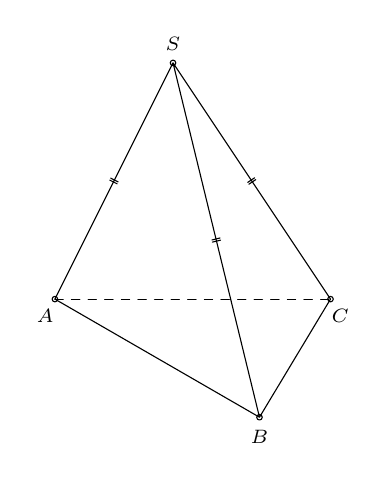
\begin{tikzpicture}[>=stealth,line join=round,line cap=round,font=\footnotesize,scale=1]
					 \path
						(0,0)  coordinate (A)
						(3.5,0) coordinate (C) 
						 (-30:3cm) coordinate (B)
						(1.5,3) coordinate (S); 
					 \draw (S)--(B)
						(S)--(A)--(B)--(C)--cycle; 
					 \draw[dashed](A)--(C);
					\foreach  \x/\y in {S/A,S/B,S/C}{
						\path (\x)--(\y) node[midway,sloped]{\tikz{\draw [shift={(-0.8pt,0)}](270:1.5pt)--(90:1.5pt) 
						 [shift={(0.8pt,0)}](270:1.5pt)--(90:1.5pt);}};
					 }
					\foreach \x/\goc in {S/90,A/240,C/-60,B/-90} 
					\draw (\x) node[shift={(\goc:7pt)},font=\scriptsize]{$\x$}  circle (1pt);
				\end{tikzpicture}
		\end{center}
		Ta có 
		\begin{eqnarray*}
			\overrightarrow{SA}\cdot \overrightarrow{BC} &=& \overrightarrow{SA}\cdot \left(\overrightarrow{SC} -  \overrightarrow{SB}\right)\\
			&=& \overrightarrow{SA}\cdot \overrightarrow{SC} - \overrightarrow{SA}\cdot \overrightarrow{SB}\\ 
			&=&SA\cdot SC\cdot \cos\widehat{ASC} - SA\cdot  SB\cdot \cos\widehat{ASB}\\
			&=& 0. 
		\end{eqnarray*}
		Suy ra $ \left(\overrightarrow{SA},\overrightarrow{BC}\right)  = 90^\circ$.
	 }
\end{ex}

% nguồn: Lop_12_Hinh_hoc_Chuong_2
\begin{ex}%[2H2H1-3]%[ma:e06888b6]
	Cho hình lăng trụ tam giác đều $ABC.A'B'C'$ có $AB  = a$ và $AA' = \sqrt{2}a$. Góc giữa hai đường thẳng $AB'$ và $BC'$ bằng
	 \choice
		{\True  $60^\circ$}
		{$45^\circ$} 
		 {$90^\circ$}
		 {$^\circ$}
	\loigiai{ 
		\begin{center}
			\begin{tikzpicture}[>=stealth,line join=round,line cap=round,font=\footnotesize,scale=1,declare function={goc=-45; a=5; b=0.45*a; h=5;}]
					 \path
						(0,0)  coordinate (A')
						(a,0) coordinate (C') 
						(goc:b)  coordinate (B')
						(0,h) coordinate (A) 
						(a,h) coordinate  (C)
						 ($(B')+(0,h)$) coordinate (B);
					 \draw[dashed] (A')--(C');
					 \draw (A')--(B')--(C')--(C)--(A)--(B)--(B')
						(A')--(A) 
						 (B)--(C)
						 (A)--(B')
						(B)--(C'); 
					\foreach \x/\goc in  {A'/-180,B'/-90,C'/0,A/-180,B/90,C/0}
					\draw (\x) node[shift={(\goc:7pt)},font=\scriptsize]{$\x$} circle  (1pt);
				\end{tikzpicture}
		\end{center}
		Ta  có
		\begin{eqnarray*}
			\overrightarrow{AB'}\cdot  \overrightarrow{BC'} &=& \left(\overrightarrow{AB} + \overrightarrow{BB'}\right)\cdot \left(\overrightarrow{BC} + \overrightarrow{CC'}\right)\\
			 &=& \overrightarrow{AB}\cdot\overrightarrow{BC} + \overrightarrow{AB}\cdot \overrightarrow{CC'} + \overrightarrow{BB'}\cdot \overrightarrow{BC} + \overrightarrow{BB'}\cdot \overrightarrow{CC'}\\
			&=& \overrightarrow{AB}\cdot \overrightarrow{BC} + \overrightarrow{AB}\cdot \overrightarrow{CC'} +  \overrightarrow{BB'}\cdot \overrightarrow{BC} + \overrightarrow{BB'}\cdot \overrightarrow{CC'}\\
			&=& -  \dfrac{a^2}{2} + 0 + 0 + 2a^2 = \dfrac{3a^2}{2}.
		\end{eqnarray*}
		 Suy ra
		\begin{eqnarray*}
			\cos\left(\overrightarrow{AB'}, \overrightarrow{BC'}\right) &=&  \dfrac{\overrightarrow{AB'}\cdot \overrightarrow{BC'}}{\left|\overrightarrow{AB'}\right|\cdot \left|\overrightarrow{BC'}\right|}\\
			&=&  \dfrac{\dfrac{3a^2}{2}}{a\sqrt{3}\cdot a\sqrt{3}} \\
			&=& \dfrac{1}{2}. 
		\end{eqnarray*}
		Vậy $\left(\overrightarrow{AB'},  \overrightarrow{BC'}\right)=60^\circ$.
	} 
\end{ex}

% nguồn: Lop_12_Hinh_hoc_Chuong_2
\begin{ex}%[2H2H1-3]%[ma:7ebadb64]
	Cho tứ diện $ABCD$ có hai mặt $ABC$ và $ABD$ là các tam giác đều. Khẳng  định nào sau đây đúng nhất.
	 \choice
		{Góc giữa $AB$ và $CD$ bằng  $60^\circ$}
		{\True $AB$ và $CD$  vuông góc với nhau}
		{$AB$ và $CD$ đồng  phẳng}
		{$AB$ và $CD$ cắt nhau} 
	 \loigiai{
		Đặt $AB = AD  = AC = a$.\\
		Ta có 
		\begin{eqnarray*}
			 \overrightarrow{CD}\cdot \overrightarrow{AB} &=&
			\left(\overrightarrow{AD} - \overrightarrow{AC}\right)\cdot  \overrightarrow{AB}\\
			&=&  \left|\overrightarrow{AD}\right|\cdot\left|\overrightarrow{AB}\right|\cos 60^\circ - \left|\overrightarrow{AB}\right|\cdot\left|\overrightarrow{AC}\right|\cos 60^\circ\\
			&=& a\cdot a\cdot \dfrac{1}{2} - a\cdot  a\cdot \dfrac{1}{2}\\
			&=&0. 
		\end{eqnarray*}
		Vậy  $\overrightarrow{AB} \perp \overrightarrow{CD}$.
	 }
\end{ex}

% nguồn: Lop_12_Hinh_hoc_Chuong_2
\begin{ex}%[2H2H1-3]%[ma:8f3170f1]
	Cho hai vectơ  $\overrightarrow{a}$, $\overrightarrow{b}$ thỏa mãn $\left|\overrightarrow{a}\right|=4$; $\left|\overrightarrow{b}\right|=3$; $\left|\overrightarrow{a}-\overrightarrow{b}\right|=4$.\\
	Gọi $\alpha$ là góc giữa hai vectơ $\overrightarrow{a}$, $\overrightarrow{b}$.  Chọn khẳng định đúng?
	\choice 
		{\True  $\cos\alpha=\dfrac{3}{8}$}
		{$\alpha=30^\circ$} 
		 {$\cos\alpha=\dfrac{1}{3}$}
		{$\alpha=60^\circ$} 
	\loigiai{ 
		 Ta có $\left(\overrightarrow{a}-\overrightarrow{b}\right)^2=\left|\overrightarrow{a}\right|^2+\left|\overrightarrow{b}\right|^2-2\overrightarrow{a}\cdot\overrightarrow{b} \Rightarrow \overrightarrow{a}\cdot\overrightarrow{b}=\dfrac{9}{2}$.\\
		 Do đó $\cos\alpha=\dfrac{\overrightarrow{a}\cdot\overrightarrow{b}}{\left|\overrightarrow{a}\right|\cdot\left|\overrightarrow{b}\right|}=\dfrac{3}{8}$.
	 }
\end{ex}

% nguồn: Lop_12_Hinh_hoc_Chuong_2
\begin{ex}%[2H2H1-3]%[ma:e4d063ea]
	Cho hình lập  phương $ABCD.EFGH$ có cạnh bằng $a$. Ta có $\overrightarrow{AB} \cdot \overrightarrow{EG}$ bằng?
	\choice 
		{$a^2\sqrt{2}$} 
		 {$a^2$}
		{$a^2\sqrt{3}$} 
		 {\True $\dfrac{a^2\sqrt{2}}{2}$}
	 \loigiai{
		\begin{center}
			\begin{tikzpicture}[>=stealth,line join=round,line cap=round,font=\footnotesize,scale=0.75,declare function={goc=210; a=3; b=5; h=5;}]
					 \path
						(0,0)  coordinate (A)--+(0,h) coordinate (E)
						(b,0)  coordinate (B)--+(0,h) coordinate (F)
						 (goc:a) coordinate (D)--+(0,h) coordinate (H)
						($(D)+(B)-(A)$) coordinate (C)--+(0,h)  coordinate (G);
					\draw[dashed] (D)--(A)--(B) 
						(A)--(E) 
						 (A)--(C)
						 (B)--(D);
					\draw  (D)--(C)--(B)--(F)--(E)--(H)--(G)--(C)
						(D)--(H) 
						(F)--(G)--(E); 
					\draw[dashed,->] (A)--(B); 
					 \draw[->] (E)--(G);
					\foreach  \x/\g in {A/35,B/0,C/-20,D/180,E/35,F/-30,G/-30,H/180}{
						\draw (\x) circle  (1pt) node[shift={(\g:7pt)},font=\footnotesize]{$\x$};}
				\end{tikzpicture}
		\end{center}
		Ta có $\overrightarrow{EF} = \overrightarrow{AB}$, $\overrightarrow{EH} =  \overrightarrow{AD}$ (do $ABFE$ và $AEHD$ là các hình chữ nhật).\\
		Suy ra 
		\begin{eqnarray*}
			\overrightarrow{AB}\cdot  \overrightarrow{EG} &=& \overrightarrow{AB} \cdot \left(\overrightarrow{EF} + \overrightarrow{EH}\right)\\
			&=& \overrightarrow{AB} \cdot \overrightarrow{EF} + \overrightarrow{AB} \cdot \overrightarrow{EH}\\ 
			&=& \overrightarrow{AB} \cdot \overrightarrow{AB}  + \overrightarrow{AB} \cdot \overrightarrow{AD}\\
			&=&  a^2 + 0\\
			&=&  a^2.
		\end{eqnarray*}
	} 
\end{ex}

% nguồn: Lop_12_Hinh_hoc_Chuong_2
\begin{ex}%[2H2H1-3]%[ma:66ffe7dd]
	Cho tứ diện $ABCD$ với $AC = \dfrac{3}{2}AD$,  $\widehat{CAB} = 60^\circ$, $\widehat{DAB} = 60^\circ$, $CD = AD$. Gọi $\varphi$ là góc giữa $AB$ và $CD$.
	Chọn khẳng định đúng? 
	\choice 
		 {\True $\cos\varphi = \dfrac{3}{4}$}
		{$\varphi =  60^\circ$}
		 {$\varphi = 30^\circ$}
		 {$\cos\varphi = \dfrac{1}{4}$}
	\loigiai{ 
		\begin{center}
			\begin{tikzpicture}[>=stealth,line join=round,line cap=round,font=\footnotesize,scale=1.5]
					 \path
						 (0,0) coordinate (B)
						(3.5,0) coordinate  (D)
						 (-35:1.5cm) coordinate (C)
						 (1.5,2) coordinate (A);
					\draw  (A)--(C)
						 (A)--(B)--(C)--(D)--cycle;
					 \draw[dashed](B)--(D);
					\foreach \x/\y in  {A/D,C/D}{
						\path (\x)--(\y) node[midway,sloped]{\tikz{\draw [shift={(-0.8pt,0)}](270:1pt)--(90:1pt) 
						[shift={(0.8pt,0)}](270:1pt)--(90:1pt);}}; 
					 }
					 \foreach \x/\goc in {A/90,B/240,D/-60,C/-90}
					\draw (\x) node[shift={(\goc:7pt)},font=\scriptsize]{$\x$} circle (1pt); 
				\end{tikzpicture}
		\end{center}
		Ta có 
		\begin{eqnarray*}
			\overrightarrow{AB}\cdot\overrightarrow{CD} &=& \overrightarrow{AB}\left(\overrightarrow{AD} - \overrightarrow{AC}\right)\\ 
			&=&\overrightarrow{AB}\cdot\overrightarrow{AD} - \overrightarrow{AB}\cdot\overrightarrow{AC}\\ 
			&=&AB\cdot  AD\cdot\cos 60^\circ - AB\cdot AC\cdot\cos 60^\circ\\
			&=&AB\cdot AD  - \dfrac{1}{2}AB\cdot AD - \dfrac{1}{2}AB\cdot AD\\
			&=&  -\dfrac{1}{4}AB\cdot CD.
		\end{eqnarray*}
		Do đó $\cos\left(\overrightarrow{AB},\overrightarrow{CD}\right) = \dfrac{\overrightarrow{AB}\cdot \overrightarrow{CD}}{\left|\overrightarrow{AB}\right|\cdot\left|\overrightarrow{CD}\right|} = \dfrac{\overrightarrow{AB}\cdot \overrightarrow{CD}}{AB\cdot CD} = \dfrac{-\dfrac{1}{4}AB\cdot CD}{AB\cdot CD} = -\dfrac{1}{4}$.\\ 
		Suy  ra $\cos\varphi = \dfrac{1}{4}$.
	} 
\end{ex}

% nguồn: Lop_12_Hinh_hoc_Chuong_2
\begin{ex}%[2H2H1-3]%[ma:af96dc09]
	Cho tứ diện $ABCD$ đều cạnh bằng $a$. Gọi $O$ là tâm đường tròn ngoại tiếp tam giác $BCD$. Góc giữa  $AO$ và $CD$ bằng bao nhiêu?
	 \choice
		{$0^\circ$} 
		{$30^\circ$} 
		{\True  $90^\circ$}
		{$60^\circ$} 
	\loigiai{ 
		\begin{center}
			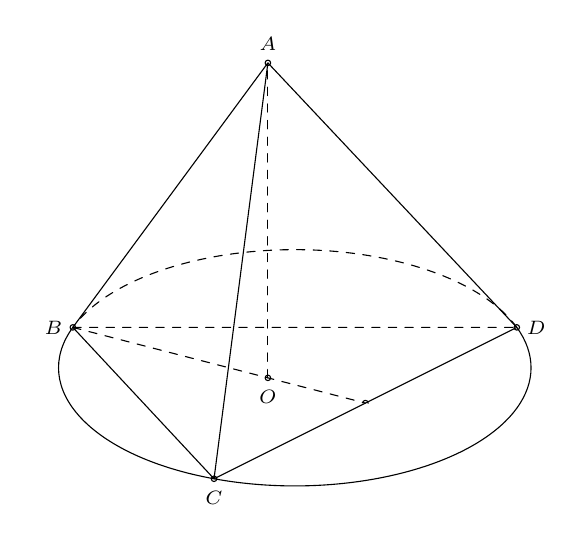
\begin{tikzpicture}[>=stealth,line join=round,line cap=round,font=\footnotesize,scale=1]
					\draw [dashed](20:3) arc (20:160: 3  and 1.5);
					\draw (160:3)  arc (160:250: 3 and 1.5) coordinate (C) arc (250:380:3 and 1.5);
					\path 
						(160:3)  coordinate (B)
						(20:3) coordinate  (D)
						 (barycentric cs:D=1,B=1,C=1) coordinate (O)
						(barycentric  cs:B=1,O=-3) coordinate (M);
					\draw[dashed] (O)--++(0,4) coordinate (A); 
					\draw (D)--(C) 
						(D)--(A)--(B)--(C)--(A); 
					\draw[dashed](B)--(D) 
						 (B)--(M) circle (1pt);
					\foreach \x/\goc  in {O/-90,A/90,B/180,C/-90,D/0}
					\draw (\x) node[shift={(\goc:7pt)},font=\scriptsize]{$\x$} circle  (1pt);
				\end{tikzpicture}
		\end{center}
		Ta  có
		\begin{eqnarray*}
			\overrightarrow{AO}\cdot \overrightarrow{CD} &=& \left(\overrightarrow{CO} - \overrightarrow{CA}\right)\cdot  \overrightarrow{CD}\\
			&=&\overrightarrow{CO}\cdot \overrightarrow{CD} - \overrightarrow{CA}\cdot  \overrightarrow{CD}\\
			 &=&CO\cdot CD\cdot \cos30^\circ - CA\cdot CD\cdot \cos60^\circ \\
			&=&\dfrac{a\sqrt{3}}{3}\cdot a\cdot  \dfrac{\sqrt{3}}{2} - a\cdot a\cdot \dfrac{1}{2}\\
			 &=& \dfrac{a^2}{2} - \dfrac{a^2}{2}\\
			&=&0. 
		\end{eqnarray*}
		Suy ra $\overrightarrow{AO}  \perp \overrightarrow{CD}$.
	 }
\end{ex}

% nguồn: Lop_12_Hinh_hoc_Chuong_2
\begin{ex}%[2H2H1-3]%[ma:aea92b8e]
	Cho tam  giác $ABC$, thì công thức tính diện tích nào sau đây là đúng nhất?
	\choice 
		 {$S = \dfrac{1}{2}\sqrt{AB^2\cdot AC^2 - BC^2}$}
		{$S =  \dfrac{1}{2}\sqrt{AB^2\cdot AC^2 + \dfrac{1}{2}\left(\overrightarrow{AB}\cdot \overrightarrow{AC}\right)^2}$}
		{$S = \dfrac{1}{2}\sqrt{AB^2\cdot AC^2 -  \dfrac{1}{2}\left(\overrightarrow{AB}\cdot \overrightarrow{AC}\right)^2}$}
		{\True $S = \dfrac{1}{2}\sqrt{AB^2\cdot AC^2 -  \left(\overrightarrow{AB}\cdot \overrightarrow{AC}\right)^2}$}
	\loigiai{ 
		 Ta có
		\begin{eqnarray*}
			 S_{ABC} &=& \dfrac{1}{2}AB\cdot AC\sin A\\
			&=& \dfrac{1}{2}\sqrt{AB^2\cdot  AC^2 \sin^2 A}\\
			&=&\dfrac{1}{2}\sqrt{AB^2\cdot AC^2  (1-\cos^2 A)}\\
			&=&\dfrac{1}{2}\sqrt{AB^2\cdot AC^2 -  \left(\overrightarrow{AB}\cdot \overrightarrow{AC}\right)^2}.
		\end{eqnarray*}
	 }
\end{ex}

% nguồn: Lop_12_Hinh_hoc_Chuong_2
\begin{ex}%[2H2H1-3]%[ma:6893d83d]
	Cho hình chóp $S.ABCD$ có đáy là hình vuông $ABCD$ cạnh bằng $a$ và các cạnh bên đều bằng $a$. Gọi $M$  và $N$ lần lượt là trung điểm của $AD$ và $SD$. Số đo của góc $(MN, SC)$ bằng
	 \choice
		{$45^\circ$} 
		 {$30^\circ$}
		 {\True $90^\circ$}
		{$60^\circ$} 
	\loigiai{ 
		Ta  có $AC = a\sqrt{2} \Rightarrow AC^2 = 2a^2 = SA^2 + SC^2 \Rightarrow \triangle SAC$ vuông tại $S$.\\
		Khi đó $\overrightarrow{NM}\cdot \overrightarrow{SC} =  \dfrac{1}{2}\overrightarrow{SA}\cdot \overrightarrow{SC} = 0 \Rightarrow \left(\overrightarrow{NM}, \overrightarrow{SC}\right) = 90^\circ$.\\
		Vậy  $(MN,SC) = 90^\circ$.
	 }
\end{ex}

% nguồn: Lop_12_Hinh_hoc_Chuong_2
\begin{ex}%[2H2H1-3]%[ma:fe8a4ccf]
	Cho hai vectơ $\overrightarrow{a},\overrightarrow{b}$ thỏa mãn $\left|\overrightarrow{a}\right|=4$;  $\left|\overrightarrow{b}\right|=3$; $\overrightarrow{a}\overrightarrow{b}=10$.\\
	Xét hai vectơ $\overrightarrow{x}=\overrightarrow{a}-\overrightarrow{b}$ $\overrightarrow{y}=\overrightarrow{a}-2\overrightarrow{b}$. Gọi $\alpha$ là góc giữa hai vectơ  $\overrightarrow{x}$, $\overrightarrow{y}$. Khi đó
	 \choice
		 {$\cos\alpha=\dfrac{-2}{\sqrt{15}}$}
		{$\cos\alpha=\dfrac{1}{\sqrt{15}}$} 
		 {$\cos\alpha=\dfrac{3}{\sqrt{15}}$}
		 {\True $\cos\alpha=\dfrac{2}{\sqrt{15}}$}
	 \loigiai{
		Ta  có $\overrightarrow{x}\cdot\overrightarrow{y}=\left(\overrightarrow{a}-2\overrightarrow{b}\right)\left(\overrightarrow{a}-\overrightarrow{b}\right)=\overrightarrow{a}^2+2\overrightarrow{b}^2-3\overrightarrow{a}\cdot\overrightarrow{b}=4$.\\
		$\left|\overrightarrow{x}\right|=\sqrt{\overrightarrow{x}^2}=\sqrt{\left(\overrightarrow{a}-2\overrightarrow{b}\right)^2}=\sqrt{\overrightarrow{a}^2+4\overrightarrow{b}^2-4\overrightarrow{a}\cdot\overrightarrow{b}}=2\sqrt{3}$.\\ 
		$\left|\overrightarrow{y}\right|=\sqrt{\overrightarrow{y}^2}=\sqrt{\left(\overrightarrow{a}-\overrightarrow{b}\right)^2}=\sqrt{\overrightarrow{a}^2+\overrightarrow{b}^2-2\overrightarrow{a}\cdot\overrightarrow{b}}=\sqrt{5}$.\\ 
		Khi đó, $\cos\alpha=\dfrac{\overrightarrow{x}\cdot  \overrightarrow{y}}{\left|\overrightarrow{x}\right|\cdot\left|\overrightarrow{y}\right|}=\dfrac{4}{2\sqrt{3}\cdot\sqrt{5}}=\dfrac{2}{\sqrt{15}}$.
	 }
\end{ex}

% nguồn: Lop_12_Hinh_hoc_Chuong_2
\begin{ex}%[2H2V1-3]%[ma:e660a1ee]
	Cho hình lăng trụ $ABC.A'B'C'$ có đáy $ABC$ là tam giác đều cạnh $a$, tam giác $A'BC$ đều nằm trong mặt phẳng vuông góc  với $(ABC)$. $M$ là trung điểm $CC'$. Tính cosin góc $\alpha$ giữa hai đường thẳng $AA'$ và $BM$.
	\choice 
		{$\cos\alpha =  \dfrac{2\sqrt{22}}{11}$}
		{\True $\cos\alpha = \dfrac{\sqrt{33}}{11}$} 
		{$\cos\alpha  = \dfrac{\sqrt{11}}{11}$}
		{$\cos\alpha =  \dfrac{\sqrt{22}}{11}$}
	 \loigiai{
		\begin{center}
			\begin{tikzpicture}[>=stealth,line join=round,line cap=round,font=\footnotesize,scale=1,declare function={goc=-45; a=5; b=0.45*a; h=4.5;}]
					 \path
						(0,0) coordinate  (A)
						(a,0) coordinate (C) 
						(goc:b)  coordinate (B)
						(3.5,h)  coordinate (A')
						 (a+3.5,h) coordinate (C')
						($(B)+(3.5,h)$) coordinate  (B')
						($(C)!0.5!(C')$) coordinate  (M)
						($(C)!0.5!(B)$)  coordinate (H);
					 \draw[dashed] (A)--(C)--(A')--(H)--(A);
					\draw  (A)--(B)--(C)--(C')--(A')--(B')--(B)
						 (A)--(A')
						 (B')--(C')
						 (A')--(B)
						 (B')--(C)
						 (B)--(M);
					\foreach \x/\goc  in {A/-180,B/-90,C/0,A'/-180,B'/90,C'/0,M/0,H/-90}
					\draw (\x)  node[shift={(\goc:7pt)},font=\scriptsize]{$\x$} circle (1pt);
				\end{tikzpicture}
		\end{center}
		 Gọi $H$ là trung điểm của $BC$.\\
		Suy  ra $AH = A'H = \dfrac{a\sqrt{3}}{2}$ và $\heva{&AH \perp BC\\&A'H \perp BC}$ $\Rightarrow BC \perp (AA'H) \Rightarrow BC \perp AA'$ hay $BC \perp BB'$.\\
		Do đó $BCC'B'$  là hình chữ nhật.\\
		Khi đó $CC' = AA' = \dfrac{a\sqrt{3}}{2}\cdot \sqrt{2} = \dfrac{a\sqrt{6}}{2}$.\\ Suy ra $BM = \sqrt{a^2 + \dfrac{a^2\cdot 6}{16}} = \dfrac{a\sqrt{22}}{4}$.\\ 
		Xét $\overrightarrow{AA'}\cdot \overrightarrow{BM} = \overrightarrow{AA'}\cdot \left(\overrightarrow{BC} + \overrightarrow{CM}\right)  = 0 + \overrightarrow{AA'}\cdot \overrightarrow{CM} = \dfrac{3a^2}{4}$.\\
		Suy ra  $\cos(AA', BM) = \dfrac{\dfrac{3a^2}{4}}{\dfrac{a\sqrt{6}}{2}\cdot \dfrac{a\sqrt{22}}{4}}= \dfrac{\sqrt{33}}{11}$.
	} 
\end{ex}


%%%%%%%%%%%%%%%% ĐÚNG/SAI %%%%%%%%%%%%%%%%

% nguồn: Lop_12_Hinh_hoc_Chuong_2
\begin{ex}%[2H2H1-3]%[ma:2dc318ae]
	Cho hình hộp chữ nhật $ABCD.A'B'C'D'$ có $AB=2a$,  $AD=3a$, $AA'=4a$.
	\begin{center}
		\begin{tikzpicture}[scale=1,>=stealth,line join=round,line cap=round,line width=1pt]
				\foreach \x/\y/\p in  {0/0/A,-1.1/-1.5/B,2.5/-1.5/C}{\path (\x,\y) coordinate (\p);}
				\path ($(A)+(C)-(B)$)  coordinate (D)
					($(A)+(0,3.2)$) coordinate (A'); 
				\foreach \x/\y in  {B/B',C/C',D/D'}{\path ($(A')+(\x)-(A)$) coordinate (\y);}
				\draw  (C)--(C')
					 (B')--(A')--(D')--(C')--(B')--(B)--(C)--(D)--(D');
				 \draw[dashed] (A')--(A)--(D)
					 (A)--(B);
				\foreach \x/\g in {A/180,B/-135,C/-45,D/0,A'/90,B'/180,C'/-10,D'/90}\fill (\x)  circle (.05)+(\g:.3) node{$\x$};
			\end{tikzpicture}
	\end{center}
	Khi  đó:
	\choiceTF 
		{\True  $\overrightarrow{AA'}+\overrightarrow{AB}+\overrightarrow{AD}=\overrightarrow{AC'}$}
		 {$\overrightarrow{AA'}\cdot\overrightarrow{AD}=12a^2$}
		{\True $\left|\overrightarrow{AB}+\overrightarrow{AD}+\overrightarrow{CC'}\right|=a\sqrt{29}$} 
		{\True Gọi $H$ là  trung điểm của $A'C$. Khi đó $\overrightarrow{AH}\cdot\overrightarrow{DB}=\dfrac{5}{2}a^2$}
	\loigiai{ 
		\begin{itemchoice}
			\itemch Đúng. Vì  ta có $\overrightarrow{AA'}+\overrightarrow{AB}+\overrightarrow{AD}=\overrightarrow{AC'}=\overrightarrow{AA'}+\overrightarrow{AC}=\overrightarrow{AC'}$
			 \itemch Sai. Vì $\overrightarrow{AA'}\cdot\overrightarrow{AD}=0$ (2 véc-tơ vuông góc với nhau)
			\itemch  Đúng. Vì $\left|\overrightarrow{AB}+\overrightarrow{AD}+\overrightarrow{CC'}\right|=\left|\overrightarrow{AC}+\overrightarrow{CC'}\right|=\left|\overrightarrow{AC'}\right|=AC'$\\
			và  $AC'=\sqrt{AC^2+CC'^2}=\sqrt{4a^2+9a^2+16a^2}=a\sqrt{29}$
			\itemch Sai.  Thiết lập hệ tọa độ như hình vẽ
			\begin{center}
				\begin{tikzpicture}[scale=1,font=\footnotesize,line join=round,line cap=round,>=stealth]
						\path (0:0) coordinate (A) 
						 ++(0:3.5) coordinate (D)
						++(-160:5) coordinate  (B)
						($(B)+(D)-(A)$) coordinate  (C)
						($(A)+(90:3)$) coordinate (A') 
						($(B)+(90:3)$) coordinate (B') 
						($(C)+(90:3)$)  coordinate (C')
						($(D)+(90:3)$)  coordinate (D')
						($(A)!1.3!(B)$) coordinate  (x)
						($(D)+(0:1)$) coordinate (y) 
						($(A')+(90:1)$) coordinate  (z);
						\draw  (C)--(C')
						 (B')--(A')--(D')--(C')--(B')--(B)--(C)--(D)--(D');
						\draw[dashed] (B)--(A)--(D) 
						(A)--(A'); 
						 \draw [->] (B)--(x);
						\draw [->] (D)--(y); 
						\draw  [->] (A')--(z);
						\foreach \x/\g  in {A/180,B/180,C/-45,D/-45,A'/150,B'/180,C'/-30,D'/0,x/180,y/-90,z/180}
						\fill (\x) circle (1pt) 
						($(\g:3.5mm)+(\x)$) node {$\x$}; 
					\end{tikzpicture}
			\end{center}
			Khi  đó ta có $A(0;0;0)$, $A'(0;0;4a)$; $C(2a;3a;0)$; $B(2a;0;0)$; $D(0;3a;0)$; $H(a;\dfrac{3a}{2};2a)$.\\
			Ta có $\overrightarrow{AH}=\left(a;\dfrac{3a}{2};2a\right)$; $\overrightarrow{DB}=\left(2a;-3a;0\right)$. Vậy $\overrightarrow{AH}\cdot\overrightarrow{DB}=2a^2-\dfrac{9}{2}a^2=-\dfrac{5}{2}a^2$. 
		\end{itemchoice}
	} 
\end{ex}

% nguồn: Lop_12_Hinh_hoc_Chuong_2
\begin{ex}%[2H2H1-3]%[ma:68da325e]
	Trong không gian, cho hai vectơ $\overrightarrow{a}$ và $\overrightarrow{b}$ cùng có độ  dài bằng $1$. Biết rằng góc giữa hai vectơ đó là $45^\circ$.
	 \choiceTF
		{\True $\overrightarrow{a}\cdot \overrightarrow{b}  = \dfrac{\sqrt{2}}{2}$}
		{\True  $\left(\overrightarrow{a}+3\overrightarrow{b}\right)\cdot\left(\overrightarrow{a}-2\overrightarrow{b}\right)=-5+\dfrac{\sqrt{2}}{2}$}
		 {$\left|\overrightarrow{a}+\overrightarrow{b}\right|=2+\sqrt{2}$}
		 {$\left|\overrightarrow{a}-\sqrt{2}\overrightarrow{b}\right|=0$}
	 \loigiai{
		\begin{itemchoice}
			\itemch $\overrightarrow{a}\cdot \overrightarrow{b} = \left|\overrightarrow{a}\right|\cdot \left|\overrightarrow{b}\right|\cos\left(\overrightarrow{a},\overrightarrow{b}\right) = \dfrac{\sqrt{2}}{2}$. 
			\itemch $\left(\overrightarrow{a}+3\overrightarrow{b}\right)\cdot\left(\overrightarrow{a}-2\overrightarrow{b}\right) = \left|\overrightarrow{a}\right|^2  + \overrightarrow{a}\cdot\overrightarrow{b} - 6\left|\overrightarrow{b}\right|^2 = 1+\dfrac{\sqrt{2}}{2}-6 = -5+\dfrac{\sqrt{2}}{2}$.
			\itemch $\left(\overrightarrow{a}+\overrightarrow{b}\right)^2 = \overrightarrow{a}^2 + 2\overrightarrow{a}\cdot \overrightarrow{b} + \overrightarrow{b}^2  = 1+2\cdot\dfrac{\sqrt{2}}{2}+1 = 2+\sqrt{2}$.\\
			Suy ra  $\left|\overrightarrow{a}+\overrightarrow{b}\right| = \sqrt{2+\sqrt{2}}$.
			\itemch $\left(\overrightarrow{a}-\sqrt{2}\overrightarrow{b}\right)^2 =  \overrightarrow{a}^2 + 2\sqrt{2}\overrightarrow{a}\cdot\overrightarrow{b} + 2\overrightarrow{b}^2 = 1+2\cdot\sqrt{2}\cdot\dfrac{\sqrt{2}}{2}+2 = 2$.\\
			Suy ra  $\left|\overrightarrow{a}-\sqrt{2}\overrightarrow{b}\right| = \sqrt{2}$.
		\end{itemchoice}
	} 
\end{ex}

% nguồn: Lop_12_Hinh_hoc_Chuong_2
\begin{ex}%[2H2V1-3]%[ma:88840d9d]
	\immini{Cho tứ diện đều $ABCD$ có cạnh bằng  $a$ và $M$ là trung điểm của $CD$.
	\choiceTF 
		 {\True $\overrightarrow{AM}\cdot \overrightarrow{CD}=0$}
		{\True $\overrightarrow{AB}\cdot  \overrightarrow{AC}=\dfrac{a^2}{2}$}
		{\True $\overrightarrow{AB}\cdot  \overrightarrow{CD}=0$}
		{$\overrightarrow{AM}\cdot  \overrightarrow{AB}=-\dfrac{a^2}{2}$}}
		{\begin{tikzpicture}[>=stealth,line join=round,line cap=round,font=\footnotesize,scale=1.5]
		\path 
			(0,0) coordinate  (B)
			 (3.5,0) coordinate (D)
			(-35:1.5cm)  coordinate (C)
			(1.5,2) coordinate  (A)
			($(C)!0.5!(D)$) coordinate  (M);
		\draw  (A)--(C)
			 (A)--(B)--(C)--(D)--cycle;
		\draw[dashed](B)--(D); 
		\foreach  \i/\j in {A/B,A/C,A/M,A/D}{
			\draw[->]  (\i)--(\j);
		} 
		 \foreach \x/\y in {D/M,C/M}{
			\path (\x)--(\y)  node[midway,sloped]{\tikz{\draw (270:1pt)--(90:1pt);}};
		} 
		\foreach \x/\goc  in {A/90,B/240,D/-60,C/-90,M/-90}
		 \draw (\x) node[shift={(\goc:7pt)},font=\scriptsize]{$\x$} circle (1pt);
	\end{tikzpicture}
		} 
	 \loigiai{
		\begin{itemchoice}
			\itemch Tam giác $ACD$ đều suy ra $AM$ vuông  góc với $CD$ nên $\overrightarrow{AM}\cdot\overrightarrow{CD}=0$.
			\itemch Ta có $\overrightarrow{AB}\cdot \overrightarrow{AC} = \left|\overrightarrow{AB}\right|\cdot  \left|\overrightarrow{AC}\right|\cos\left(\overrightarrow{AB},\overrightarrow{AC}\right) = AB\cdot AC\cdot \cos 60^\circ = a\cdot a\cdot \cos 60^\circ = \dfrac{a^2}{2}$.
			\itemch Ta có  $AM$, $BM$ là trung tuyến của các tam giác đều $ACD$, $BCD$ nên $\heva{&AM \perp CD\\& MB \perp CD.}$\\
			Suy ra $\overrightarrow{AM}\cdot \overrightarrow{CD} = \overrightarrow{MB}\cdot \overrightarrow{CD} = 0$.\\ 
			Do đó $\overrightarrow{AB}\cdot  \overrightarrow{CD} = \left(\overrightarrow{AM}+\overrightarrow{MB}\right)\cdot \overrightarrow{CD} = \overrightarrow{AM}\cdot \overrightarrow{CD} + \overrightarrow{MB}\cdot\overrightarrow{CD}=0$.
			\itemch Ta có $\overrightarrow{AM} =  \dfrac{1}{2}\left(\overrightarrow{AC}+\overrightarrow{AD}\right)$.
			\\ Suy ra $\overrightarrow{AB}\cdot \overrightarrow{AM} = \overrightarrow{AB}\cdot \dfrac{1}{2} \left(\overrightarrow{AC}+\overrightarrow{AD}\right) = \dfrac{1}{2}\left(\overrightarrow{AB}\cdot \overrightarrow{AC} + \overrightarrow{AB}\cdot \overrightarrow{AD}\right) = \dfrac{1}{2}\cdot \left(\dfrac{a^2}{2} +  \dfrac{a^2}{2}\right) = \dfrac{a^2}{2}$.
		\end{itemchoice}
	 }
\end{ex}


%%%%%%%%%%%%%%%% TRẢ LỜI NGẮN %%%%%%%%%%%%%%%%

% nguồn: Lop_12_Hinh_hoc_Chuong_2
\begin{bt}%[2H2V1-3]%[ma:9b769aef]
	Trong không gian, cho hình lập phương $ABCD.A'B'C'D'$ biết  rằng $\overrightarrow{AN}=-4\overrightarrow{AB}+k\overrightarrow{AA'}-2\overrightarrow{AD}$ $(k \in \mathbb{R})$ và $\overrightarrow{AM}=2\overrightarrow{AB}+\overrightarrow{AA'}-3\overrightarrow{AD}$. Tìm giá trị $k$ thích hợp để $\overrightarrow{AN} \perp \overrightarrow{AM}$.
	\shortans{2} 
	\loigiai{ 
		\begin{center}
			\begin{tikzpicture}[scale=0.6,font=\footnotesize,line join=round,line cap=round]
					\def\h{4} 
					\foreach  \x\y\t in {0/0/A,-1/-1.1/B,2.6/-1.1/C}
					 \coordinate (\t) at (\x,\y);
					\coordinate (D) at  ($(A)+(C)-(B)$);
					\coordinate  (A') at ($(A)+(0,3.2)$);
					\coordinate (B')  at ($(B)+(0,3.2)$);
					\coordinate (C') at  ($(C)+(0,3.2)$);
					\coordinate (D') at ($(D)+(0,3.2)$); 
					\draw  (B')--(A')--(D')--(C')--(B')--(B)--(C)--(D)--(D')
						 (C')--(C);
					\draw[dashed](B)--(A)--(D) 
						 (A)--(A');
					\foreach \t/\g in  {A/170,B/-150,C/-70,D/0,A'/100,B'/170,C'/-20,D'/50}
					\draw (\t)  circle (1pt)
						 node[shift={(\g:7pt)}]{$\t$};
				\end{tikzpicture}
		\end{center}
		Vì $ABCD.A'B'C'D'$ là hình lập  phương nên $AB=AA'=AD$\\
		Các vectơ $\overrightarrow{AB}$, $\overrightarrow{AA'}$, $\overrightarrow{AD}$  đôi một vuông góc với nhau.\\
		Do đó: $\overrightarrow{AB} \cdot \overrightarrow{AA'}=0$; $ \overrightarrow{AB} \cdot \overrightarrow{AD}=0$; $ \overrightarrow{AA'}  \cdot \overrightarrow{AD}=0$.\\
		Để $\overrightarrow{AN} \perp \overrightarrow{AM}$ thì $\overrightarrow{AN}  \cdot \overrightarrow{AM}=0 $
		\begin{eqnarray*}
			&\Leftrightarrow& \left(-4\overrightarrow{AB}+k\overrightarrow{AA'}-2\overrightarrow{AD}\right)  \cdot \left(2\overrightarrow{AB}+\overrightarrow{AA'}-3\overrightarrow{AD}\right)=0\\
			&\Leftrightarrow&-8AB^2+kAA'^2+6AD^2=0 \text{ mà }  (AB=AA'=AD)\\
			&\Leftrightarrow&-8AB^2+kAA'^2+6AB^2=0 \Leftrightarrow(-8+k+6)AB^2=0\Leftrightarrow-8+k+6=0\\ 
			&\Leftrightarrow& k=2. 
		\end{eqnarray*}
	Vậy $k=2$ thì  $\overrightarrow{AN}\perp \overrightarrow{AM}.$}
\end{bt}

% nguồn: Lop_12_Hinh_hoc_Chuong_2
\begin{bt}%[2H2V1-3]%[ma:0b602022]
	Trong không gian, cho hình chóp $S.ABCD$ có đáy là hình bình hành tâm $O$, $M$ là điểm  thay đổi trên $SO$. Tỉ số $\dfrac{SM}{SO}$ sao cho $P=MS^2+MA^2+MB^2+MC^2+MD^2$ nhỏ nhất là bao nhiêu?
	 \shortans{0,8}
	 \loigiai{
		\begin{center}
			\begin{tikzpicture}[scale=1.2,font=\footnotesize,line join=round,line cap=round,>=stealth]
					\coordinate[label=below left:$A$] (A) at (0,0); 
					\coordinate[label=below right:$B$] (B) at  (3,0);
					\coordinate[label=right:$C$] (C) at ($(B)+(1.5,1.5)$); 
					\coordinate[label=above  left:$D$] (D) at ($(A)+(1.5,1.5)$);
					\coordinate  (O) at ($(A)!0.5!(C)$);
					\fill (O) circle  (1pt) node[below] {$O$};
					\coordinate[label=above:$S$]  (S) at ($(O)+(-0.4,3)$);
					 \coordinate (I) at ($(S)!0.8!(O)$);
					\fill (I)  circle (1pt) node[left] {$I$};
					\draw (A)--(B)--(C); 
					 \draw (S)--(A)
						(S)--(B) 
						(S)--(C); 
					\draw[dashed]  (S)--(D)
						(A) -- (C) -- (D) -- (B) 
						(A)  -- (D);
					 \draw[dashed] (S)--(O);
					 \foreach \pt in {A,B,C,D,S}
					\fill (\pt) circle  (1.5pt);
				\end{tikzpicture}
		\end{center}
		Gọi $I$ là điểm thỏa mãn  $\overrightarrow{SI}=\dfrac{4}{5}\overrightarrow{SO}$.\\
		Suy ra \begin{eqnarray*}
		P  &=&\left(\overrightarrow{MI}+\overrightarrow{IS}\right)^2+\left(\overrightarrow{MI}+\overrightarrow{IA}\right)^2+\left(\overrightarrow{MI}+\overrightarrow{IB}\right)^2+\left(\overrightarrow{MI}+\overrightarrow{IC}\right)^2+\left(\overrightarrow{MI}+\overrightarrow{ID}\right)^2\\
		&=&5MI^2+IS^2+IA^2+IB^2+IC^2+ID^2+2\overrightarrow{MI}\left(\overrightarrow{IS}+\overrightarrow{IA}+\overrightarrow{IB}+\overrightarrow{IC}+\overrightarrow{ID}\right)\\ 
		&=&5MI^2+IS^2+IA^2+IB^2+IC^2+ID^2+2\overrightarrow{MI}\left(\overrightarrow{IS}+4\overrightarrow{IO}+\overrightarrow{OA}+\overrightarrow{OB}+\overrightarrow{OC}+\overrightarrow{OD}\right)\\ 
		 &=&5MI^2+IS^2+IA^2+IB^2+IC^2+ID^2+2\overrightarrow{MI}\left(\overrightarrow{IS}+4\overrightarrow{IO}\right)\\
		 &=&5MI^2+IS^2+IA^2+IB^2+IC^2+ID^2.\\
\end{eqnarray*} Vậy $P_{\text{ min}}$ khi $M=I \Rightarrow \dfrac{SM}{SO}=\dfrac{4}{5}=0{,}8$.}
\end{bt}

% nguồn: Lop_12_Hinh_hoc_Chuong_2
\begin{bt}%[2H2V1-3]%[ma:c2f5a29f]
	Trong không gian, cho tứ diện $S.ABC$ có $SA=SB=SC=AB=AC=2$, $ BC=2\sqrt{2}$. Hãy tính  $\overrightarrow{SC}\cdot\overrightarrow{AB}$.
	\shortans{-2} 
	\loigiai{ 
		\begin{center}
			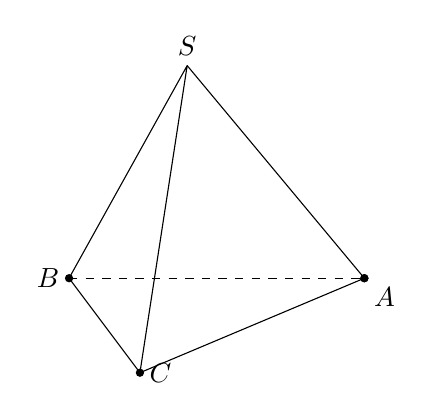
\begin{tikzpicture}[scale=1.5,line join=round]
					\coordinate[label=above:$S$]  (S) at (0,1.8);
					\coordinate[label=left:$B$] (B)  at (-1,0);
					 \coordinate[label=below right:$A$] (A) at (1.5,0);
					\coordinate[label=right:$C$]  (C) at (-0.4,-0.8);
					\draw (S) -- (A) -- (C)  -- (B) -- cycle (S) -- (C);
					\draw[dashed]  (B) -- (A);
					\foreach \pt in {A,B,C,A} 
					\fill (\pt) circle  (1pt);
				\end{tikzpicture}
		\end{center}
		Ta có $BC^2=SB^2+SC^2 \ (2.2=2+2) \Rightarrow \triangle SBC$ vuông cân tại  $S$.\\
		 Mặt khác $SA=AC=SC=2 \Rightarrow \triangle SAC$ là tam giác đều.\\
		$\overrightarrow{SC}\cdot\overrightarrow{AB}=\overrightarrow{SC}\cdot\left(\overrightarrow{SB} - \overrightarrow{SA}\right)=\overrightarrow{SC}\cdot\overrightarrow{SB} - \overrightarrow{SC}\cdot\overrightarrow{SA}=0 - SC\cdot SA\cdot\cos \widehat{ASC}=-2\cdot2\cdot\cos 60^{\circ}=-\dfrac{2^2}{2}=-2$.\\ 
	Vậy $\overrightarrow{SC}\cdot\overrightarrow{AB}=-2$.} 
\end{bt}


%%%%%%%%%%%%%%%% TỰ LUẬN %%%%%%%%%%%%%%%%

% nguồn: Lop_12_Hinh_hoc_Chuong_2
\begin{bt}%[2H2H1-3]%[ma:5ea05a3f]
	Cho hình chóp  tứ giác đều $S.ABCD$ có độ dài tất cả các cạnh bằng $a$. Tính các tích vô hướng sau:
	\begin{enumerate}
		\item $\overrightarrow{AS}\cdot \overrightarrow{BC}$. 
		 \item $\overrightarrow{AS}\cdot \overrightarrow{AC}$.
	\end{enumerate}
	\loigiai{ 
		\begin{center}
			\begin{tikzpicture}[>=stealth,line join=round,line cap=round,font=\footnotesize,scale=1]
					\def\a{4} 
					 \def\h{4.5}
					\path (0:0) coordinate (A) 
						++(0:\a) coordinate (D) 
						 ++(-130:\a/2) coordinate (C)
						($(A)+(C)-(D)$) coordinate  (B)
						(intersection of A--C and B--D) coordinate  (O)
						($(O)+(90:\h)$)  coordinate (S);
					 \draw[dashed](B)--(A)--(D)
						(A)--(C) 
						 (B)--(D)
						 (S)--(O);
					 \draw (B)--(C)--(D)
						 (B)--(S)
						(C)--(S) 
						(D)--(S); 
					 \draw[dashed,->](A)--(S);
					 \draw[dashed,->](A)--(C);
					\draw[->](B)--(C); 
					\foreach \x/\g  in {A/135,B/-135,C/-45,D/45,S/90,O/-90}
					\fill (\x) circle  (1.5pt)
						($(\g:3mm)+(\x)$) node {$\x$}; 
					\draw pic[draw,angle radius=3mm]{right angle=D--O--S}; 
				\end{tikzpicture}
		\end{center}
		\begin{enumerate}
			\item $\triangle SAD$ có ba cạnh bằng nhau nên  là tam giác đều, suy ra $\widehat{SAD} = 60^\circ$.
			Tứ giác $ABCD$ là  hình vuông nên $\overrightarrow{AD} = \overrightarrow{BC}$.\\
			Suy ra $\left(\overrightarrow{AS},\overrightarrow{BC}\right) = \left(\overrightarrow{AS},\overrightarrow{AD}\right) = \widehat{SAD}  = 60^\circ$.\\
			Do đó, $\overrightarrow{AS}.\overrightarrow{BC} = \left|\overrightarrow{AS}\right|\cdot\left|\overrightarrow{BC}\right|\cdot\cos 60^\circ = a\cdot a\cdot\dfrac{1}{2}  = \dfrac{a^2}{2}$.
			\item Tứ giác $ABCD$ là hình vuông có độ dài mỗi cạnh là $a$ nên độ dài đường chéo  $AC$ là $\sqrt{2}a$.
			\\ Tam  giác $SAC$ có $SA=SC=a$ và $AC=\sqrt{2}a$ nên tam giác $SAC$ vuông cân tại $S$.\\
			Suy  ra $\widehat{SAC}=45^\circ$.\\
			Do  đó $\overrightarrow{AS}\cdot \overrightarrow{AC}=\left|\overrightarrow{AS}\right|\cdot \left|\overrightarrow{AC}\right|\cdot \cos \widehat{SAC}=a\cdot \sqrt{2}a\cdot \dfrac{\sqrt{2}}{2}=a^2$.
		\end{enumerate}
	 }
\end{bt}

% nguồn: Lop_12_Hinh_hoc_Chuong_2
\begin{bt}%[2H2H1-3]%[ma:e7060c1a]
	Cho hình lăng  trụ tứ giác đều $ABCD.A'B'C'D'$ có độ dài mỗi cạnh đáy bằng $1$ và độ dài cạnh bên bằng $2$. Hãy tính góc giữa các cặp vectơ sau đây và tính tích vô hướng của mỗi cặp vectơ đó.
	\begin{enumerate}
		\item  $\overrightarrow{AA'}$ và $\overrightarrow{CC'}$
		\item $\overrightarrow{AA'}$ và $\overrightarrow{BC}$ 
		\item $\overrightarrow{AC}$  và $\overrightarrow{B'A'}$
	\end{enumerate}
	\loigiai{ 
		\begin{center}
			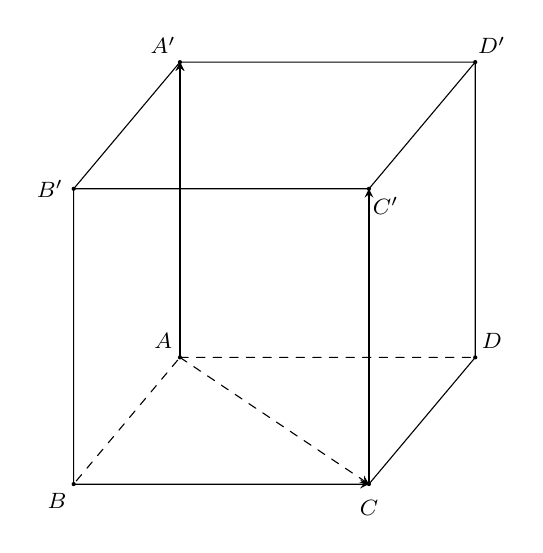
\begin{tikzpicture}[>=stealth,line join=round,line cap=round,font=\footnotesize,scale=0.75]
					\def\r{-130} 
					 \def\c{5}
					\def\d{2.8} 
					 \path
						(0:0)  coordinate (A)++(0:\c)
						coordinate (D)++(90:\c) coordinate  (D')
						(A)++(\r:\d) coordinate (B)++(0:\c) coordinate (C)++(90:\c) coordinate  (C')
						(A)++(90:\c)  coordinate (A')++(\r:\d) coordinate (B');
					\draw  (A')--(B')--(B)--(C)--(D)--(D')--(A')
						 (B')--(C')--(D');
					\draw[dashed] (A')--(A)--(B) 
						 (A)--(D);
					 \draw[dashed,->](A)--(C);
					 \draw[dashed,->](A)--(A');
					 \draw[->](C)--(C');
					\draw[->](A)--(A'); 
					 \draw[->](B)--(C);
					 \foreach \p / \r in {A/135,B/-135,D/45,A'/135,B'/180,D'/45,C/-90,C'/-45}
					\fill (\p) circle  (1pt) node[shift={(\r:3mm)}]{$\p$};
				\end{tikzpicture}
		\end{center}
		\begin{enumerate}
			\item Vì $AA'\parallel  CC'$ nên hai vectơ $\overrightarrow{AA'}$ và $\overrightarrow{CC'}$ cùng hướng.\\
			Do  đó $\overrightarrow{AA'}\cdot \overrightarrow{CC'}=\left|\overrightarrow{AA'}\right|\cdot\left|\overrightarrow{CC'}\right|=2\cdot 2=4$.
			\item  Vì $A'ADD'$ là hình chữ nhật nên $\widehat{A'AD}=90^\circ$.\\
			Vì $ABCD$ là hình  vuông nên $\overrightarrow{BC}=\overrightarrow{AD}$.\\
			Do đó  $\left(\overrightarrow{AA'},\overrightarrow{BC}\right)=\left(\overrightarrow{AA'},\overrightarrow{AD}\right)=\widehat{A'AD}=90^\circ$.\\
			Ta có $\overrightarrow{AA'}\cdot \overrightarrow{BC}=\overrightarrow{AA'}\cdot \overrightarrow{AD}=\left|\overrightarrow{AA'}\right|\cdot\left|\overrightarrow{AD}\right|\cdot \cos\left(\overrightarrow{AA'},\overrightarrow{AD}\right)=2\cdot  1\cdot \cos90^\circ=0$.
			\item Vì $A'ABB'$ là  hình chữ nhật nên $\overrightarrow{B'A'}=\overrightarrow{BA}$.\\
			Mặt khác  $ABCD$ là hình vuông nên $\widehat{CAB}=45^\circ$ và $AC=\sqrt{2}$.\\
			Ta có  $\overrightarrow{AC}\cdot \overrightarrow{B'A'}=-\overrightarrow{AC}\cdot\overrightarrow{AB}=-\left|\overrightarrow{AC}\right|\cdot\left|\overrightarrow{AB}\right|\cdot \cos\left(\overrightarrow{AC},\overrightarrow{AB}\right)=-\sqrt{2}\cdot 1\cdot \cos45^\circ=-1$.
		\end{enumerate}
	 }
\end{bt}

% nguồn: Lop_12_Hinh_hoc_Chuong_2
\begin{bt}%[2H2H1-3]%[ma:024e9fc0]
	Cho tứ  diện $ABCD$ có $AC$ và $BD$ cùng vuông góc với $AB$. Gọi $M$, $N$ lần lượt là trung điểm của hai cạnh $AB$, $CD$. Chứng minh rằng:
	\begin{listEX}[2]
		\item  $\overrightarrow{MN} = \dfrac{1}{2}\left(\overrightarrow{AC} + \overrightarrow{BD}\right)$
		\item $\overrightarrow{MN}\cdot \overrightarrow{AB}  = 0$
	\end{listEX}
	\loigiai{ 
		\begin{enumerate}
			 \item\immini{Ta có $\overrightarrow{MN}=\overrightarrow{MA}+\overrightarrow{AC}+\overrightarrow{CN}$ và $\overrightarrow{MN}=\overrightarrow{MB}+\overrightarrow{BD}+\overrightarrow{DN}$.\\
			Do  đó $2\overrightarrow{MN}=\left(\overrightarrow{MA}+\overrightarrow{MB}\right)+\left(\overrightarrow{AC}+\overrightarrow{BD}\right)+\left(\overrightarrow{CN}+\overrightarrow{DN}\right)$.\\
			Vì $M$, $N$ lần lượt là trung điểm của $AB$, $CD$ nên\\ $\overrightarrow{MA}+\overrightarrow{MB}=\overrightarrow{0}$  và $\overrightarrow{CN}+\overrightarrow{DN}=\overrightarrow{0}$.\\
			Suy ra $2\overrightarrow{MN}=\overrightarrow{AC}+\overrightarrow{BD}$, hay  $\overrightarrow{MN}=\dfrac{1}{2}\left(\overrightarrow{AC}+\overrightarrow{BD}\right)$.
			 }{
			\begin{tikzpicture}[line join=round,line cap=round,font=\footnotesize,scale=1,>=stealth]
					\def  \r{2.5}
					 \path
						 (0,0) coordinate (B)
						(60:0.7*\r) coordinate  (A)
						 (0:\r) coordinate (D)
						 (-40:0.5*\r) coordinate (C)
						($(A)!0.5!(B)$) coordinate (M) 
						($(C)!0.5!(D)$) coordinate  (N);
					 \draw[-stealth](A)--(B);
					\draw[-stealth](A)--(C); 
					\draw[-stealth](A)--(D); 
					\draw (B)--(C)--(D); 
					\draw[dashed] (B)--(D); 
					\draw[dashed,-stealth] (M)--(N); 
					\foreach \x/\g in {A/90,B/180,C/-90,D/0,M/150,N/-30}\fill (\x) circle (1pt)+(\g:.3) node{$\x$}; 
				\end{tikzpicture}
			 }
			\item Từ  giả thiết, ta có $\overrightarrow{AC}\cdot \overrightarrow{AB}=0$ và $\overrightarrow{BD}\cdot \overrightarrow{AB}=0$.\\
			Vì vậy $\overrightarrow{MN}\cdot \overrightarrow{AB}=\dfrac{1}{2}\left(\overrightarrow{AC}+\overrightarrow{BD}\right)\cdot  \overrightarrow{AB}=\dfrac{1}{2}\overrightarrow{AC}\cdot \overrightarrow{AB}+\dfrac{1}{2}\overrightarrow{BD}\cdot \overrightarrow{AB}=0$.
		\end{enumerate}
	 }
\end{bt}

% nguồn: Lop_12_Hinh_hoc_Chuong_2
\begin{bt}%[2H2H1-3]%[ma:6209360a]
	Một chiếc xe  đang kéo căng sợi dây cáp $AB$ trong công trường xây dựng, trên đó đã thiết lập hệ toạ độ $Oxyz$ như hình vẽ dưới với độ dài đơn vị trên các trục tọa độ bằng $1$ m. Tìm được tọa độ của vectơ $\overrightarrow{AB}=\left(a;b;c\right)$. Khi đó tính $a+c$
	\begin{center}
		\begin{tikzpicture}[line join = round,line cap=round,>=stealth,font=\footnotesize,scale=0.5]
				\path (0,0)  coordinate (O)
					 (5,0) coordinate (H)
					(-2,-2) coordinate  (K)
					($(K)+(H)-(O)$) coordinate  (B)
					($(O)+(0,3.6)$)  coordinate (A);
				\foreach \x/\y in{K/x,H/y,A/z} 
				\draw[->,line width=1pt,scale=1.5]  (O)--(\x)--($(O)!1.4!(\x)$) node[right]{$\y$};
				\draw[pattern=crosshatch] (-0.2,0) rectangle (0.3,4) 
					 (-2.5,3.6) rectangle (0.3,4);
				\draw[pattern=crosshatch,rotate=-50,xshift=-3cm,yshift=2.4cm] 
					(-0.2,0) rectangle (0.3,1.5); 
				\draw[cyan,line  width=4pt] (O)--(A);
				\foreach \p/\r  in {A/0,K/180,H/90,B/70,O/-90}
				\fill (\p)  circle (1.2pt) node[shift={(\r:3mm)}]{$\p$};
				 \draw[dashed] (O)--($(O)-(1,0)$);
				\draw[<->,line width=2pt] ($(O)-(1,0)$)--($(A)-(1,0)$)  node[pos=0.5,left]{$10$ m};
				 \draw[line width=1pt] (O)--(B) node[pos=0.5,below,rotate=-35]{$15$ m};
				 \draw (K)--(B)--(H)
					(B)--(O); 
				\draw pic[draw,angle radius=6mm] {angle  = B--O--H};
				\draw  ($(O)+(1,-0.25)$) node{$30^\circ$};
				\draw[->,line  width=2pt] (A)--(B);
				 \draw (B) node[xshift=0.5cm,yshift=-0.5cm]{
			\begin{tikzpicture}[line join = round,line cap=round,>=stealth,font=\footnotesize,scale=0.4]
					\draw[rotate=-65,scale=1,line width=5pt,xshift=1.8cm,yshift=2.4cm] (0.7,-1.5) ellipse (0.4cm and  0.3cm);
					 \fill[green!80] (0,0)--(0,-1)--(1,-2)--(2,-2)--(2,-1)--(1,0)--cycle;
					 \draw[rotate=-65,scale=1,line width=5pt] (1,-0.4) ellipse (0.4cm and 0.3cm);
					\draw[rotate=-65,scale=1,,line width=5pt,xshift=1.4cm,yshift=1.5cm] (0.7,-1.5) ellipse  (0.4cm and 0.3cm);
				\end{tikzpicture}
		}; 
	\end{tikzpicture}
\end{center}
\loigiai{ 
	Ta có $\overrightarrow{OA}=10\vec{k}\Rightarrow A\left(0;0;10\right)$ và $OH=OB\cdot\cos 30^{\circ} =\dfrac{15\sqrt{3} }{2} $; $OK=OB\cdot\cos \left(90^{\circ} -30^{\circ}  \right)=\frac{15}{2}.$\\
	$\Rightarrow B\left(\dfrac{15}{2};\dfrac{15\sqrt{3} }{2};0\right)\Rightarrow \overrightarrow{AB}=\left(\dfrac{15}{2};\dfrac{15\sqrt{3}  }{2};-10\right)$. Vậy $a+c=2{,}5$.
} 
\end{bt}

% nguồn: Lop_12_Hinh_hoc_Chuong_2
\begin{bt}%[2H2H1-3]%[ma:9e5b6afb]
	Trong không gian với hệ tọa độ $Oxyz$ cho ba điểm $M\left(2; 3; -1\right)$, $N\left(-1;1;1\right)$ và $P\left(1;m-1; 2\right)$. Tìm $m$ để tam giác $MNP$ vuông tại  $N$.
	 \loigiai{
	 $\overrightarrow{MN}\left(-3;-2;2\right);\overrightarrow{NP}\left(2; m-2;1\right)$.\\
	Tam giác $MNP$ vuông tại $N\Leftrightarrow \overrightarrow{MN}\cdot \overrightarrow{NP}=0\Leftrightarrow  -6-2\left(m-2\right)+2=0\Leftrightarrow m-2=-2\Leftrightarrow m=0$.
	} 
\end{bt}

% nguồn: Lop_12_Hinh_hoc_Chuong_2
\begin{bt}%[2H2H1-3]%[ma:eedd8300]
	Cho hình lập phương $ABCD.A'B'C'D'$ có cạnh  bằng $5$.
	\begin{enumerate}
		\item Tìm góc giữa các cặp vectơ sau: $\overrightarrow{AC}$ và $\overrightarrow{AB}$;  $\overrightarrow{AC}$ và $\overrightarrow{B'D'}$; $\overrightarrow{AC}$ và $\overrightarrow{CD}$; $\overrightarrow{AD'}$ và $\overrightarrow{BD}$.
		\item Tính các tích vô hướng  $\overrightarrow{AC}\cdot \overrightarrow{AB}$; $\overrightarrow{AC}\cdot\overrightarrow{B'D'}$; $\overrightarrow{AD'}\cdot\overrightarrow{BD}$
		\item Chứng minh $\overrightarrow{AC'}$  vuông góc với $\overrightarrow{BD}$.
	\end{enumerate}
	\loigiai{ 
		\begin{center}
			\begin{tikzpicture}[>=stealth,line join=round,line cap=round,font=\footnotesize,scale=0.75]
					 \def\r{-130}
					 \def\c{5}
					 \def\d{2.8}
					\path 
						(0:0)  coordinate (A)++(0:\c)
						 coordinate (D)++(90:\c) coordinate (D')
						(A)++(\r:\d) coordinate (B)++(0:\c) coordinate (C)++(90:\c)  coordinate (C')
						(A)++(90:\c) coordinate (A')++(\r:\d) coordinate  (B')
						($(A)!2!(C)$) coordinate  (E);
					 \draw (A')--(B')--(B)--(C)--(D)--(D')--(A')
						 (D')--(B')--(C')--(D')
						(C)--(C')--(A') 
						 (C)--(E);
					 \draw[dashed] (A')--(A)--(B)
						 (A)--(D)
						(C)--(A)--(C') 
						(B)--(D); 
					\foreach \p /  \r in {A/135,B/-135,D/45,A'/135,B'/180,D'/45,C/-90,C'/-45,E/-90}
					\fill (\p) circle  (1pt) node[shift={(\r:3mm)}]{$\p$};
				\end{tikzpicture}
		\end{center}
		\begin{enumerate}
			\item Ta có $\left(\overrightarrow{AC}, \overrightarrow{AB}\right) = \widehat{CAB} = 45^\circ$; $\left(\overrightarrow{AC}, \overrightarrow{B'D'}\right) =  \left(\overrightarrow{AC}, \overrightarrow{BD}\right) = 90^\circ$;\\
			$\left(\overrightarrow{AC}, \overrightarrow{CD}\right) = \left(\overrightarrow{CE}, \overrightarrow{CD}\right)  = 180^\circ - 45^\circ = 135^\circ$ ($E$ là điểm đối xứng của $A$ qua $C$).\\
			Do $\overrightarrow{AD'} = \overrightarrow{BC'} \Rightarrow  \left(\overrightarrow{AD'}, \overrightarrow{BD}\right) = \left(\overrightarrow{BC'}, \overrightarrow{BD}\right) = \widehat{C'BD}$.\\
			Mà $\triangle C'BD$ đều nên $\widehat{C'BD} =  60^\circ$.
			\item Ta có $AC  = BD = B'D' = 5\sqrt{2}$ suy ra
			\begin{itemize}
				\item $\overrightarrow{AC}\cdot\overrightarrow{AB}  = AC\cdot AB\cdot \cos 45^\circ = 25$
				\item Do $\overrightarrow{AC}\perp\overrightarrow{B'D'}$  nên $\overrightarrow{AC}\cdot \overrightarrow{B'D'} = 0$.
				\item $\overrightarrow{AD'}\cdot \overrightarrow{BD} = AD'\cdot  BD\cdot \cos 60^\circ = 5\sqrt{2}\cdot 5\sqrt{2}\cdot \dfrac{1}{2} = 25$.
			\end{itemize}
			\item Ta cần  chứng minh $\overrightarrow{AC'}\cdot \overrightarrow{BD} = 0$.\\
			Ta có $\overrightarrow{AC'}  = \overrightarrow{AB} + \overrightarrow{AD} + \overrightarrow{AA'}$ và $\overrightarrow{BD} = \overrightarrow{AD} - \overrightarrow{AB}$ nên
			\begin{eqnarray*}
				\overrightarrow{AC'}\cdot \overrightarrow{BD} &=& \left(\overrightarrow{AB} + \overrightarrow{AD}  + \overrightarrow{AA'})\cdot(\overrightarrow{AD} - \overrightarrow{AB}\right)\\
				 &=& \overrightarrow{AB}\cdot\overrightarrow{AD} - \overrightarrow{AB}^2 + \overrightarrow{AD}^2 - \overrightarrow{AD}\cdot \overrightarrow{AB} + \overrightarrow{AA'}\cdot \overrightarrow{AD} - \overrightarrow{AA'}\cdot \overrightarrow{AB}\\ &=& 5^2 - 5^2 = 0.
			\end{eqnarray*}
			Suy ra $\overrightarrow{AC'}\perp \overrightarrow{BD}$ (điều phải chứng  minh).
		\end{enumerate}
	 }
\end{bt}

% nguồn: Lop_12_Hinh_hoc_Chuong_2
\begin{bt}%[2H2V1-3]%[ma:a6cee080]
	Cho biết $A$ (đơn vị: J) sinh bởi lực $\overrightarrow{F}$ tác dụng lên một vật được tính bằng công thức $A = \overrightarrow{F}\cdot\overrightarrow{d}$ trong đó $\overrightarrow{d}$ là vectơ biểu thị độ dịch chuyển của vật (đơn vị: mét) khi chịu tác dụng của lực $\overrightarrow{F}$. Một chiếc xe có khối lượng $1{,}5$ tấn đang đi xuống trên một đoạn đường dốc có góc nghiêng $5^\circ$ so với phương ngang. Tính công sinh ra bởi trọng lực $\overrightarrow{P}$ khi xe đi hết đoạn đường dốc dài $30$ m  (làm tròn kết quả đến hàng đơn vị). Biết rằng trọng lực $\overrightarrow{P}$ được xác định bởi công thức $\overrightarrow{P} = m\cdot \overrightarrow{g}$, với $m$ (đơn vị: kg) là khối lượng của vật và $\overrightarrow{g}$ là gia tốc rơi tự do có độ lớn $g = 9{,}8$ m/s$^2$.
	 \loigiai{
		\begin{center}
			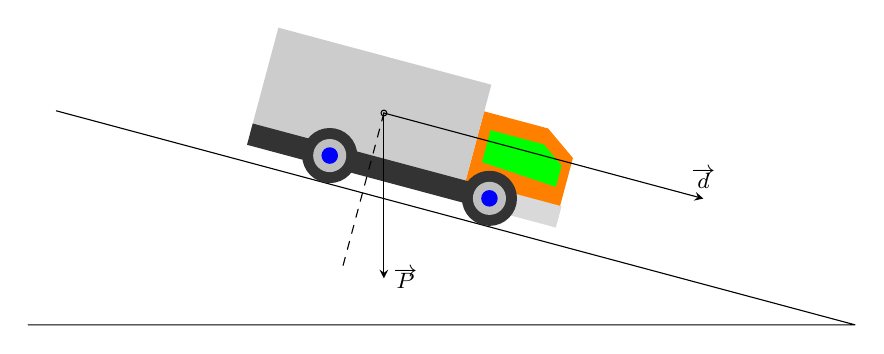
\begin{tikzpicture}[scale=0.7,>=stealth,line join=round,line cap=round,font=\footnotesize]
					 \def\g{15}
					\path  (0,0) coordinate (O)
						 +(180:15) coordinate (O1)
						+({180-\g}:15) coordinate  (O2)
						 +({180-\g}:7) coordinate (B)
						 +({180-\g}:10) coordinate (C)
						(B)++({90-\g}:1.5)++({180-\g}:2.25)  coordinate (M);
					\draw  (O1)--(O)--(O2);
					 \fill [orange] (B)++({90-\g}:.5)++({180-\g}:.5)--++({90-\g}:1.5)--++({-\g}:1.2)--++(-50:.7)--++({-\g-90}:1.2)--cycle;
					\fill [green]  (B)++({90-\g}:1.1)++({180-\g}:.3)--++({90-\g}:.6)--++({-\g}:1)--++(-50:.5)--++({-\g-90}:.4)--cycle;
					\fill [gray!40] (B)++({90-\g}:.5)++({180-\g}:.5)--++({90-\g}:2)--++({180-\g}:4)--++({-\g-90}:2)--cycle; 
					 \fill [black!80] (B)++({90-\g}:.7)--++({180-\g}:4.5)--++({-\g-90}:.4)--++({-\g}:4.5)--cycle;
					\fill [gray!30]  (B)++({90-\g}:.7)--++({-\g}:1.3)--++({-\g-90}:.4)--++({180-\g}:1.3)--cycle;
					 \draw [dashed] (M)--++({-\g-90}:3);
					\draw [->] (M)--++(-90:3)  node [right] {$\overrightarrow{P}$};
					\draw [->] (M)--++({-\g}:6)  node [above] {$\overrightarrow{d}$};
					\draw (M) circle  (1.5pt);
					\foreach \x in {B,C}{ 
						\fill [black!80] (\x)++({90-\g}:.5)  circle (.5);
						\fill  [gray!50] (\x)++({90-\g}:.5) circle (.3);
						\fill [blue] (\x)++({90-\g}:.5)  circle (.15);
					} 
				\end{tikzpicture}
		\end{center}
		Ta có $1{,}5$ tấn = $1\,500$ kg.\\ 
		Độ lớn của trọng lực tác dụng lên xe là $\left|\overrightarrow{P}\right| = m\cdot\left|\overrightarrow{g}\right|  = 1\,500\cdot 9{,}8 = 14\,700$ (N).\\
		Vectơ $\overrightarrow{d}$ biểu thị độ dịch chuyển của  xe có độ dài là $\left|\overrightarrow{d}\right| = 30$ (m) và $\left(\overrightarrow{P},\overrightarrow{d}\right) = 90^\circ - 5^\circ = 85^\circ$.\\
		Công  sinh ra bởi trọng lực khi xe đi hết đoạn đường dốc là
		$$A = \overrightarrow{P}\cdot \overrightarrow{d} =  \left|\overrightarrow{P}\right|\cdot\left|\overrightarrow{d}\right|\cdot\cos\left(\overrightarrow{P},\overrightarrow{d}\right) = 14\,700\cdot 30\cdot \cos85^\circ \approx 38\,436 \text{ (J)}.$$
	 }
\end{bt}

% nguồn: Lop_12_Hinh_hoc_Chuong_2
\begin{bt}%[2H2V1-3]%[ma:8a6fa449]
	Cho tứ diện đều $ABCD$ cạnh $a$. Gọi $M$ là trung điểm của $BC$. Tính $\cos\left(\overrightarrow{AB},\overrightarrow{DM}\right)$ 
	\loigiai{ 
		 Xét tứ diện $ABCD$ cạnh $a$, có $DM =AM = \dfrac{a\sqrt{3}}{2}$.
		\begin{eqnarray*}
			\overrightarrow{AB}\cdot\overrightarrow{DM} &=& \overrightarrow{AB}\cdot \left(\overrightarrow{AM} -  \overrightarrow{AD}\right)\\
			&=&\overrightarrow{AB}\cdot\overrightarrow{AM} -  \overrightarrow{AB}\cdot\overrightarrow{AD}\\
			&=&\left|\overrightarrow{AB}\right|\cdot \left|\overrightarrow{AM}\right|\cos\left(\overrightarrow{AB}, \overrightarrow{AM}\right) - \left|\overrightarrow{AB}\right|\cdot  \left|\overrightarrow{AD}\right|\cos\left(\overrightarrow{AB}, \overrightarrow{AD}\right)\\
			&=&a\cdot\dfrac{a\sqrt{3}}{2}\cdot\dfrac{\sqrt{3}}{2} - a\cdot a\cdot  \dfrac{1}{2}\\
			&=&\dfrac{a^2}{4}. 
		\end{eqnarray*}
		Do đó $\cos\left(\overrightarrow{AB}, \overrightarrow{DM}\right) = \dfrac{\overrightarrow{AB}\cdot \overrightarrow{DM}}{\left|\overrightarrow{AB}\right|\cdot\left|\overrightarrow {DM}\right|} = \dfrac{AM.DM}{a\cdot\dfrac{a\sqrt{3}}{2}} = \dfrac{\dfrac{\sqrt{3}}{2}a^2}{\dfrac{a\sqrt{3}}{2}} = \dfrac{2}{a^2}$.\\ 
		Vậy $\cos\left(\overrightarrow{AB},  \overrightarrow{DM}\right) = \dfrac{\sqrt{3}}{6}$.
	} 
\end{bt}
